\begin{ParaColumn}[\bisection*{Experimental Predictions}{实验预测}]
    
    To assess the proposed model and the criteria of static liquefaction, experimental results (e.g., undrained triaxial test) are required for validation. There are two kinds of loading modes for undrained triaxial tests: (1) load-controlled loading mode, and (2) deformation-controlled loading mode. In load-controlled triaxial tests, instability occurs along with the sudden increase of strain rate, whereas in deformation-controlled tests, prefailure strain softening takes places under the same other conditions \citep{Chu2001}. Although both phenomena are different, the mechanism that governs the onset of instability is the same and could be predicted by the same criteria \citep{Chu2001, Chu2009}. Because this study focused on the onset of static liquefaction instability and the soil behavior at postpeak stage is beyond the study’s scope, only the deformation-controlled triaxial tests were analyzed.

    \switchcolumn

    为了评估建议的模型和静态液化标准,需要使用实验结果(例如不排水的三轴试验)进行验证。 不排水的三轴试验有两种加载方式:(1)荷载控制的加载方式和(2)变形控制的加载方式。 在载荷控制的三轴试验中,不稳定性随应变速率的突然增加而发生,而在变形控制的试验中,失效前的应变软化在相同的其他条件下发生\citep{Chu2001}。 尽管两种现象都不同,但控制不稳定性发作的机制是相同的,并且可以用相同的标准进行预测\citep{Chu2001, Chu2009}。 由于本研究的重点是静态液化不稳定性的发生,并且峰后阶段的土体行为超出了研究范围,因此仅分析了变形控制的三轴试验。

    \switchcolumn*[\bisubsection*{Isotropically Consolidated Undrained Triaxial Tests}{各向同性固结不排水三轴试验}]

    The proposed constitutive model and the instability criteria were used to predict the results of the isotropically consolidated undrained triaxial tests of \citet{Doanh1997}. The specimen, which was 70 mm in diameter and 70 mm in height, was made of Hostun RF sand with minimum void ratio $e_{\min} = 0.648$ and maximum void ratio $e_{\max} = 1.041$. The void ratios of the specimen after isotropical consolidation were 0.883, 0.875, and 0.854. The initial effective consolidation pressures of the tests were 100, 200, and 300 kPa.

    \switchcolumn

    提出的本构模型和不稳定性标准被用来预测\citet{Doanh1997}的各向同性固结不排水三轴试验的结果。 直径为70毫米,高度为70毫米的样品是由Hostun RF砂制成的,其最小孔隙比$e_{\min} = 0.648$,最大孔隙比$e_{\max} = 1.041$。 各向同性固结后,试样的孔隙比分别为0.883、0.875和0.854。 试验的初始有效固结压力为100、200和300 kPa。

    \CrossColumnText{
        \begin{figure}[htb]
    \centering
    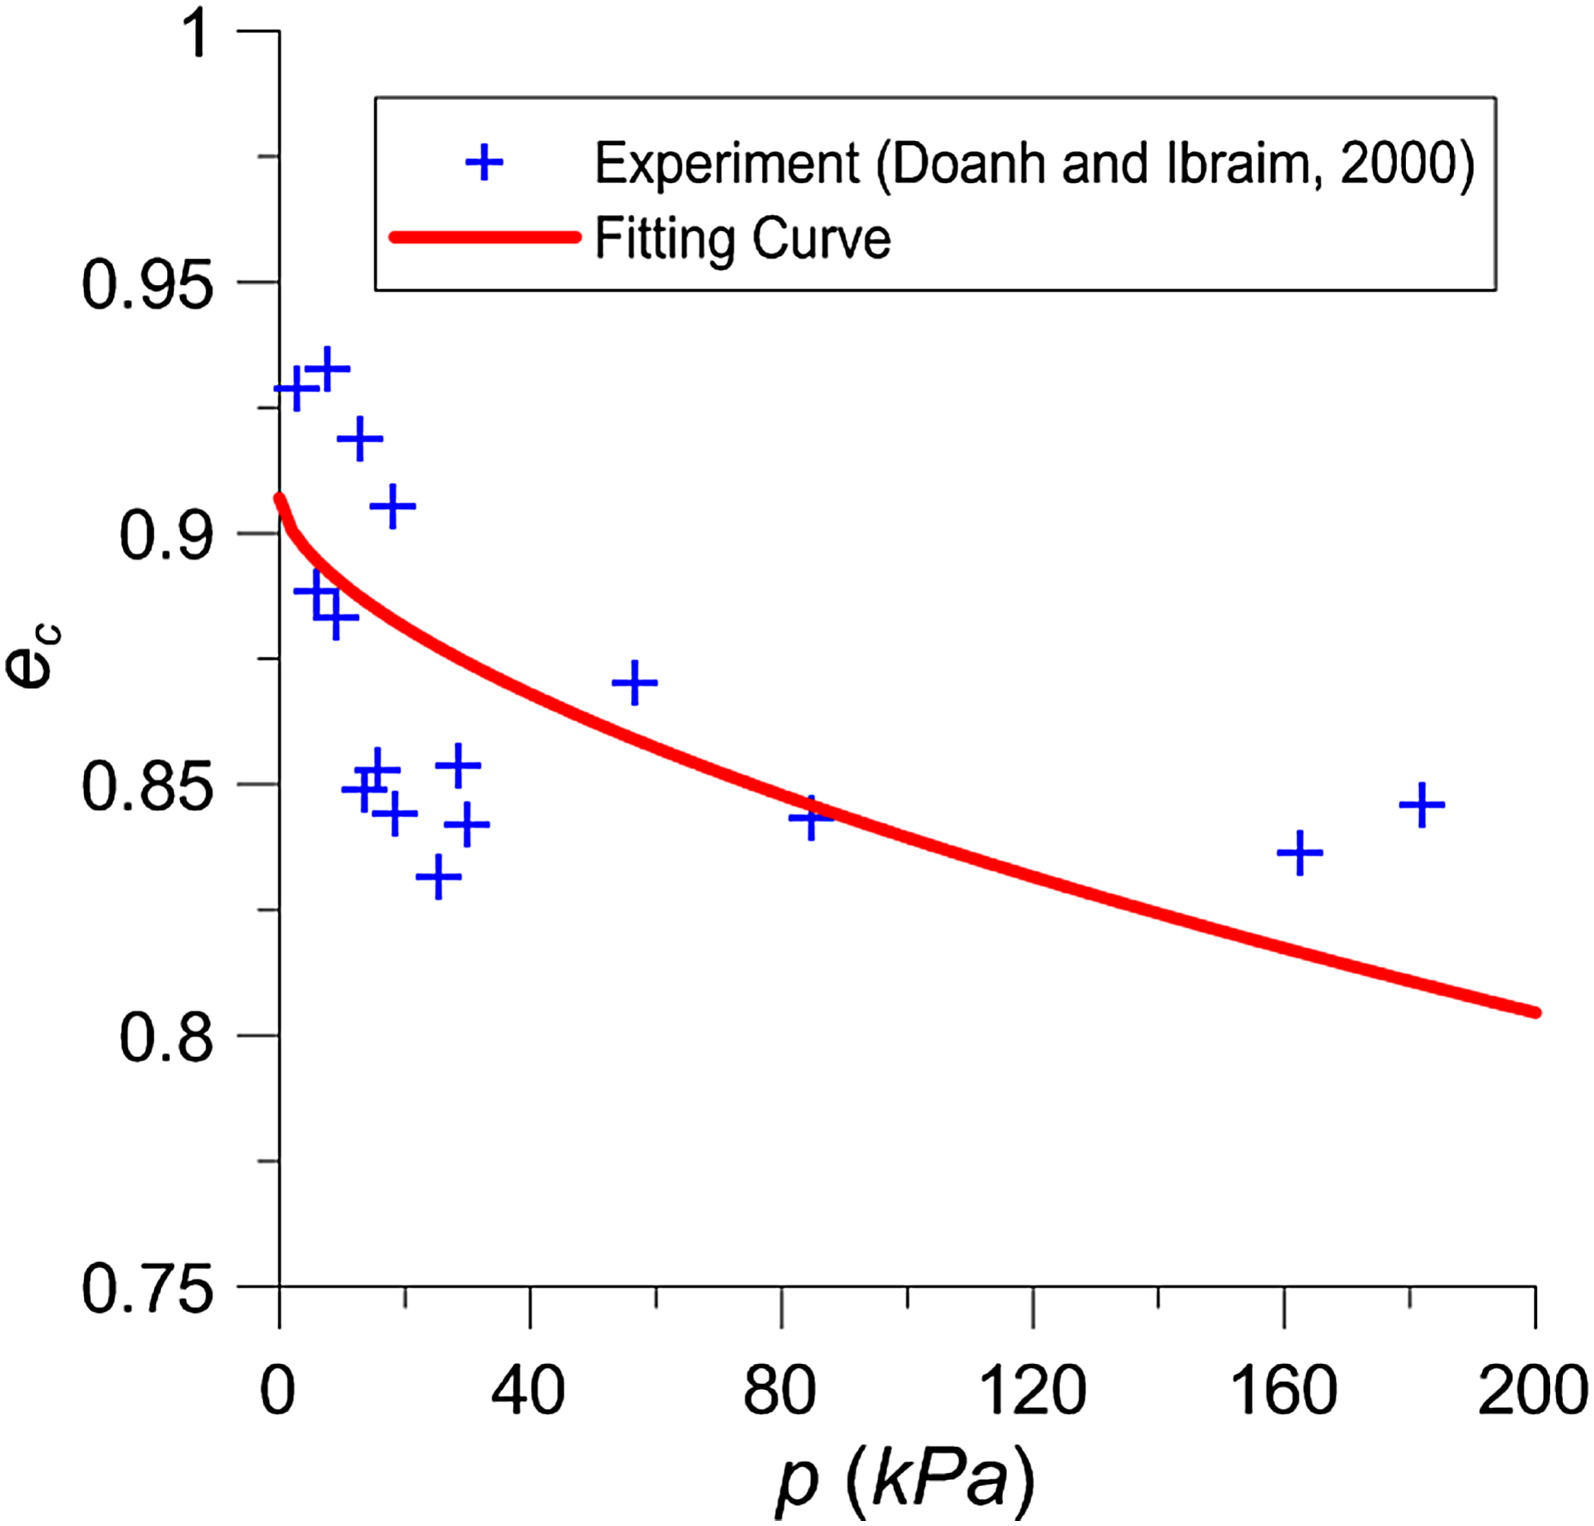
\includegraphics[width=.5\textwidth]{figures/figure3.jpg}
    \bicaption{The  $e_c-p$  curve at critical state (experimental data from \citet{Doanh2000})}{临界状态下的$e_c-p$曲线(来自\citet{Doanh2000}的实验数据)}
    \label{figure:3}
\end{figure}
    }
    \switchcolumn*

    The elastic parameter $G_{0}$ is a regression constant and could be determined by fitting a series of independent small-strain test data (e.g., from bender element tests) using \enautoref{equation:14}; Poisson's ratio $\nu$ could be determined by \enautoref{equation:14} when the bulk modulus was known. The parameter $M_{c s}$ and parameters $\lambda_{c}, e_{c 0},$ and $\xi$ were determined by fitting the experimental data of the stress ratio and $e-p$ data at the critical state. The obtained $e_{c}-p$ curve of Hostun $\mathrm{RF}$ sand (Doanh and Ibraim 2000 ) is shown in \enautoref{figure:3} The $n_{b}$ could be determined by \enautoref{equation:5} from the measured data of $\psi$ and $M$ at the phase-transformation state, $n_{d}$ could be determined by \enautoref{equation:7} from the measured data of $\psi$ and $M$ at the drained peak stress state, and $d_{0}$ could be determined by the $\varepsilon_{v}-\varepsilon_{q}$ curve from the drained triaixal test. A fitting parameter $A$ could be obtained by fitting the stress-strain relationships.

    \switchcolumn

    弹性参数$G_{0}$是一个回归常数,可以通过使用等式拟合一系列独立的小应变试验数据(例如,来自弯曲元试验)使用\cnautoref{equation:14}来确定。当体积模量已知时泊松比$\nu$可由\cnautoref{equation:14}确定。参数$M_{cs}$和参数$\lambda_{c}$,$e_{c0}$和$\xi$是通过在临界状态下拟合应力比和$e-p$的实验数据来确定的。获得的Hostu n$\mathrm{RF}$砂土的$e_{c}-p$曲线\citep{Doanh2000}如\cnautoref{figure:3}所示。$n_{b}$可以由\cnautoref{equation:5}确定。从相变状态下的$\psi$和$M$的测量数据中,可以用\cnautoref{equation:7}从在排水状态下的$\psi$和$M$的测量数据确定$n_{d}$峰值应力状态,$d_{0}$可以通过排水三轴试验的$\varepsilon_{v}-\varepsilon_{q}$曲线确定。通过拟合应力应变关系可以获得拟合参数$A$。

    \switchcolumn*

    After all the material parameters were calibrated (listed in \cnautoref{table:1}), the behavior of the specimen was predicted by deformation-controlled loading. As shown in \enautoref{figure:4}, the predicted effective stress path under undrained loading process compared very well with the experiments. The predicted effective stress-strain relationship and pore-water pressure are shown in \enautoref{figure:5}; the deviatoric shear stress rapidly increased to the peak, and then decreased along with the continuous increase in pore-water pressure. During the loading process, the determinant of the symmetric elastoplastic modulus tensor and second-order work were calculated. As shown in \enautoref{figure:6}, both values vanished simultaneously at the peak of the deviatoric stress, which indicates that the static liquefaction started when the soil entered into the potentially unstable state. The evolution of the hardening modulus Hp is shown in \enautoref{figure:7}; the static liquefaction occurred at the hardening stage of the soil. The difference between these results and those of \citet{Andrade2009}, in which static liquefaction occurred at the softening regime of the soil, is due to the adoption of a different kind of constitutive model.

    \switchcolumn

    校准所有材料参数(在\cnautoref{table:1}中列出)后,通过变形控制载荷预测样品的行为。如\cnautoref{figure:4}所示,在不排水的加载过程中预测的有效应力路径与实验结果非常吻合。预测的有效应力应变关系和孔隙水压力如\cnautoref{figure:5}所示。偏剪应力迅速增加到峰值,然后随着孔隙水压力的不断增加而减小。在加载过程中,计算了对称弹塑性模量张量的决定因素和二阶功。如\cnautoref{figure:6}所示,这两个值在偏应力峰值时同时消失,这表明当土体进入潜在不稳定状态时,静态液化开始。硬化模量Hp的变化如\cnautoref{figure:7}所示。静态液化发生在土体的硬化阶段。这些结果与\citet{Andrade2009}的结果之所以不同,是由于采用了另一种本构模型,在土体的软化状态下发生了静态液化。

    \CrossColumnText{
        \begin{table}[htbp]
    \centering
    \bicaption{Material Parameters Used in the Simulation [Experimental Data from \citet{Doanh1997} and \citet{Chu2008}]}{模拟中使用的材料参数[实验数据来自\citet{Doanh1997}以及\citet{Chu2008}]}
    \label{table:1}
    \begin{tabularx}{\textwidth}{lll}
        \toprule
        Material parameters & Istropically consolidated undrained triaxial tests & $K_0$-consolidated undrained triaxial tests \\
        \midrule
        $G_0$ & 125 & 30 \\
        $\nu$ & 0.15 & 0.05 \\
        $M_{cs}$ & 1.0 & 1.35\\
        $\lambda_c$ & 0.078 & 0.098 \\
        $e_{c0}$ & 0.907 & 0.972 \\
        $\xi$ & 0.6 & 0.4 \\
        $n_b$ & 1.1 & 1.1 \\
        $n_d$ & 3.5 & 3.5 \\
        $d_0$ & 0.88 & 0.88 \\
        $A$ & 0.001 & 0.003 \\
        \bottomrule
    \end{tabularx}
\end{table}
        \begin{figure}[p]
    \centering
    \begin{minipage}[b]{.48\textwidth}
        \begin{figure}[H]
            \centering
            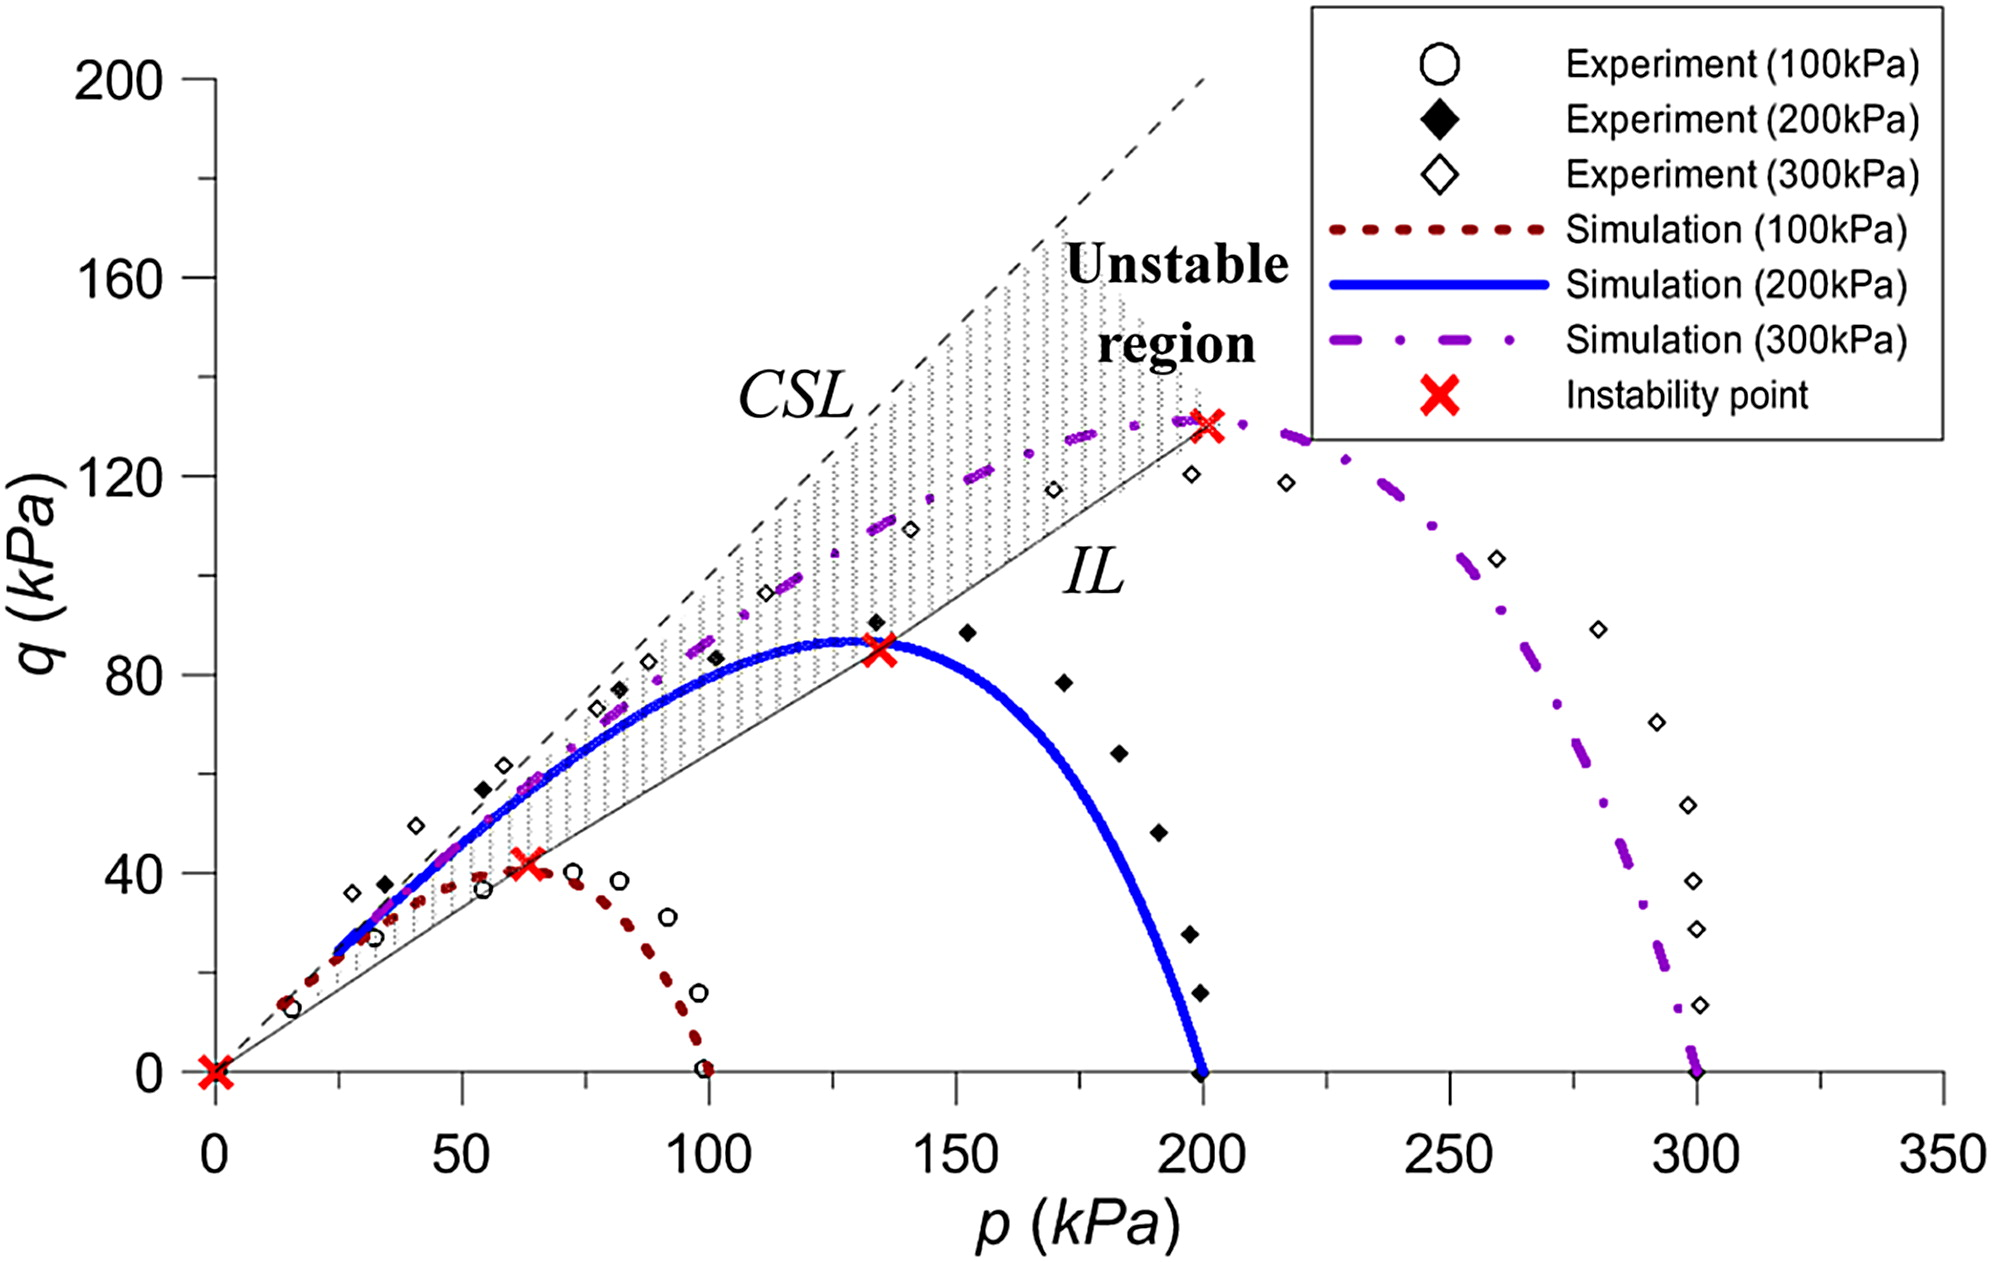
\includegraphics[width=.75\textwidth]{figures/figure4.jpg}
            \bicaption{Stress path of isotropically consolidated undrained triaxial test (experimental data from \citet{Doanh1997})}{各向同性固结不排水三轴试验的应力路径(实验数据来自\citet{Doanh1997})}
            \label{figure:4}
        \end{figure}
        \begin{figure}[H]
            \centering
            \addtocounter{figure}{1}
            \subfigure[determinant of the symmetric part of the elastoplastic modulus tensor 弹塑性模量张量的对称部分的行列式的演变]{
                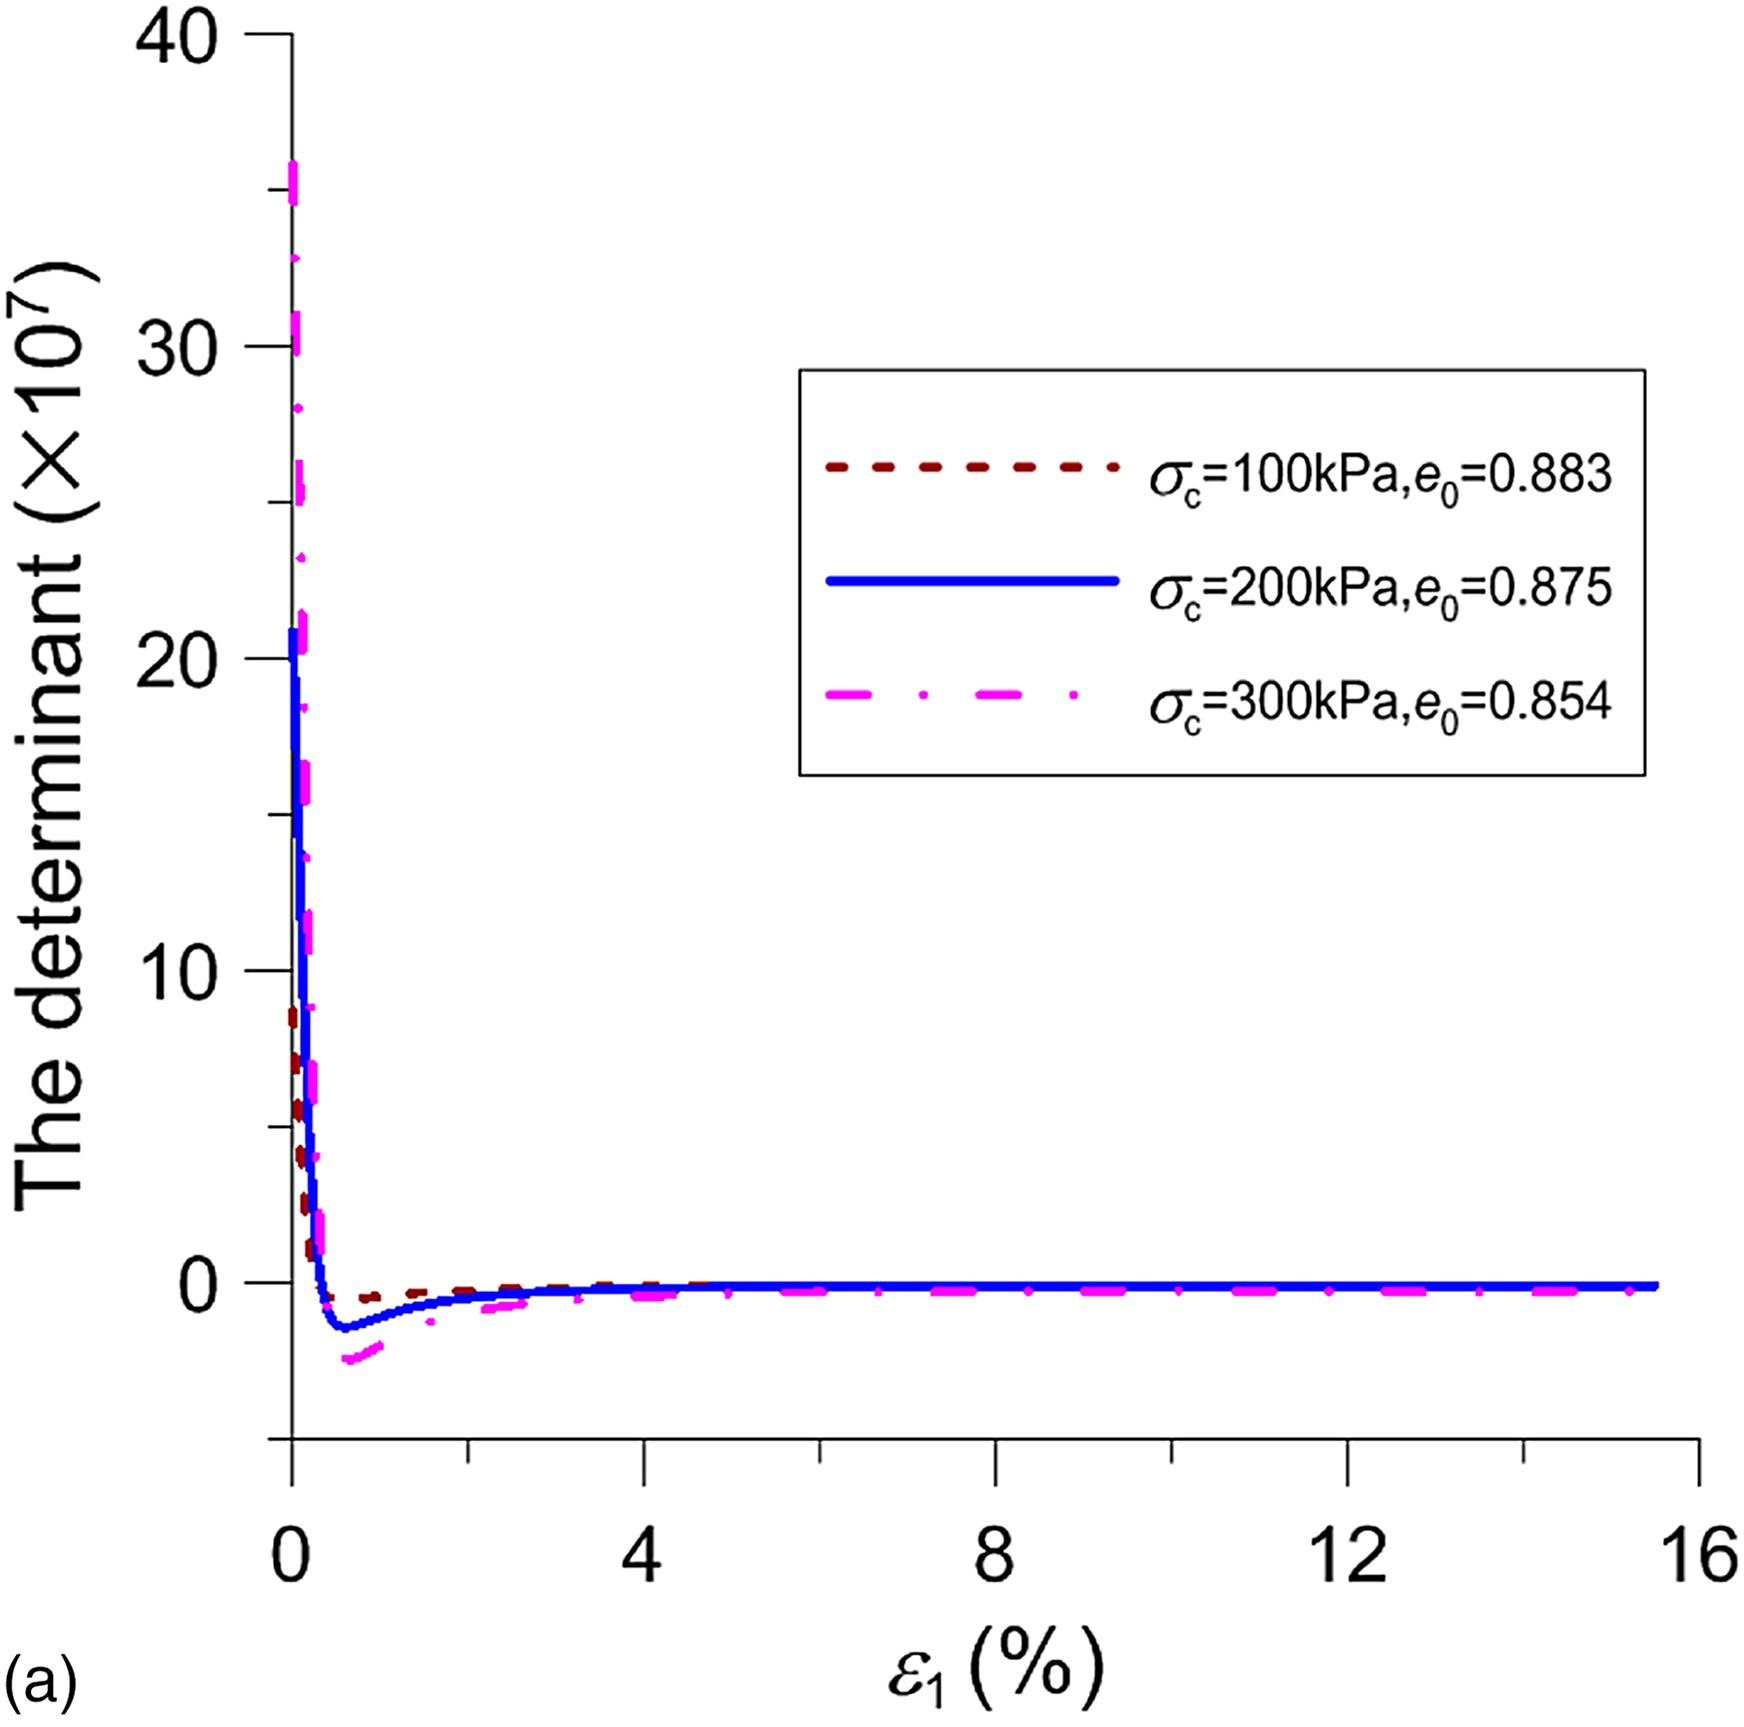
\includegraphics[width=.75\textwidth]{figures/figure6a.jpg}
                \label{figure:6a}
            }
            \subfigure[evolution of second-order work 二阶功]{
                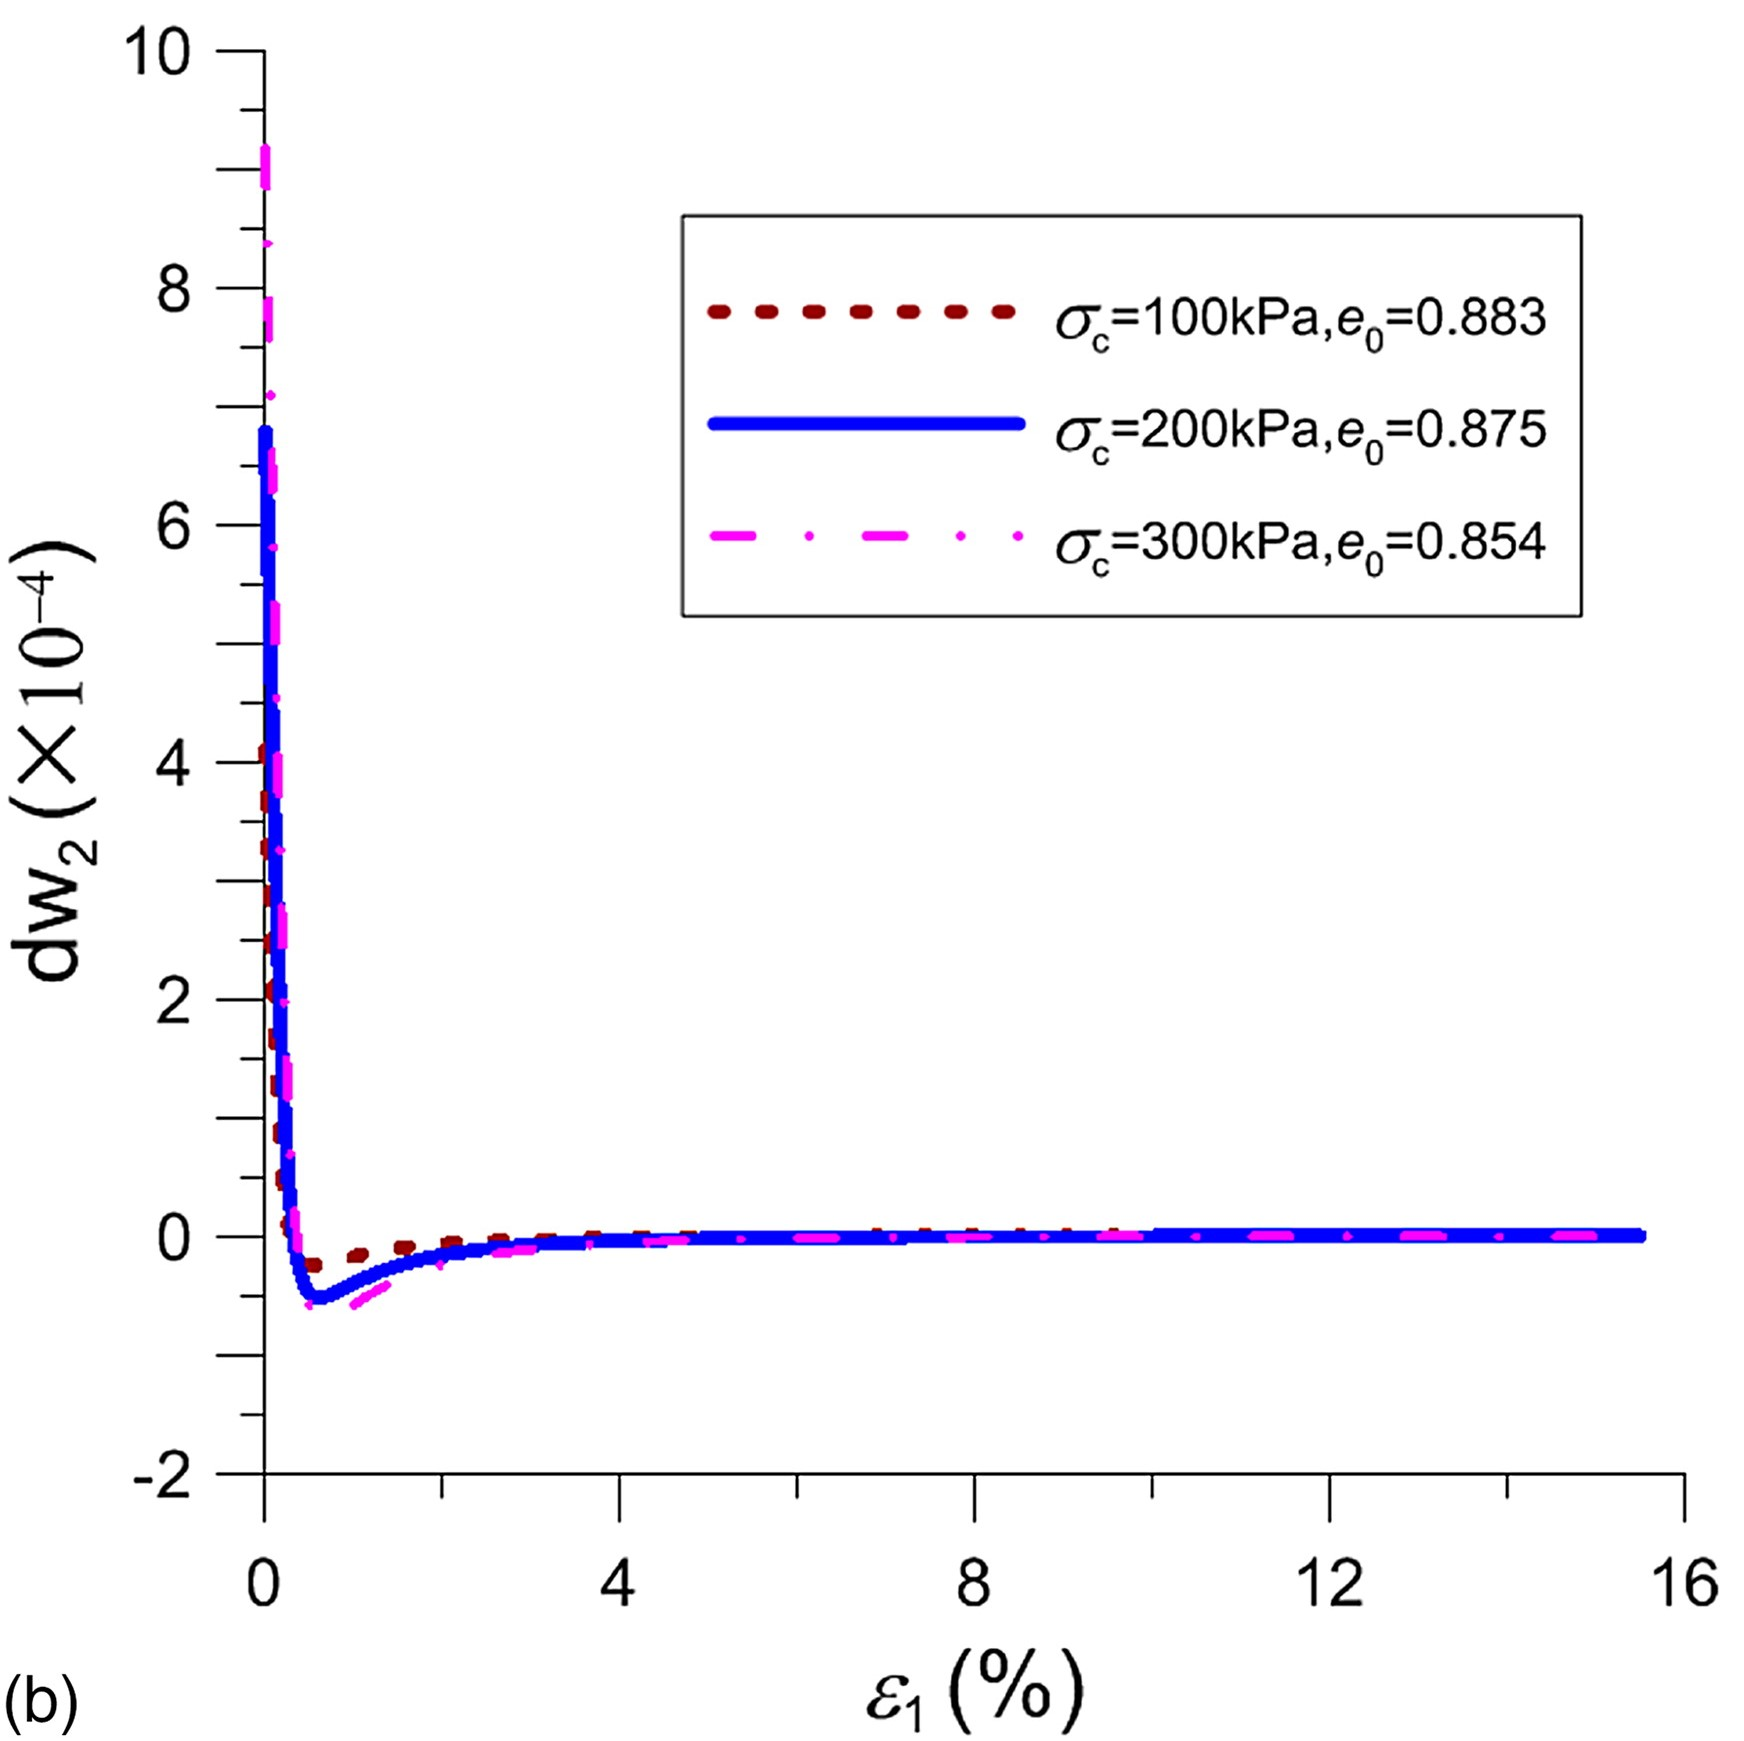
\includegraphics[width=.75\textwidth]{figures/figure6b.jpg}
                \label{figure:6b}
            }
            \bicaption{Evolution of determinant of the symmetric part of the elastoplastic modulus tensor and second-order work}{弹塑性模量张量的对称部分的行列式的和二阶功的演变}
            \label{figure:6}
        \end{figure}
    \end{minipage}
    \hspace{0.02\textwidth}
    \begin{minipage}[b]{.48\textwidth}
        \begin{figure}[H]
            \centering
            \addtocounter{figure}{-2}
            \subfigure[deviatoric stress, major principal strain 偏应力,主应变]{
                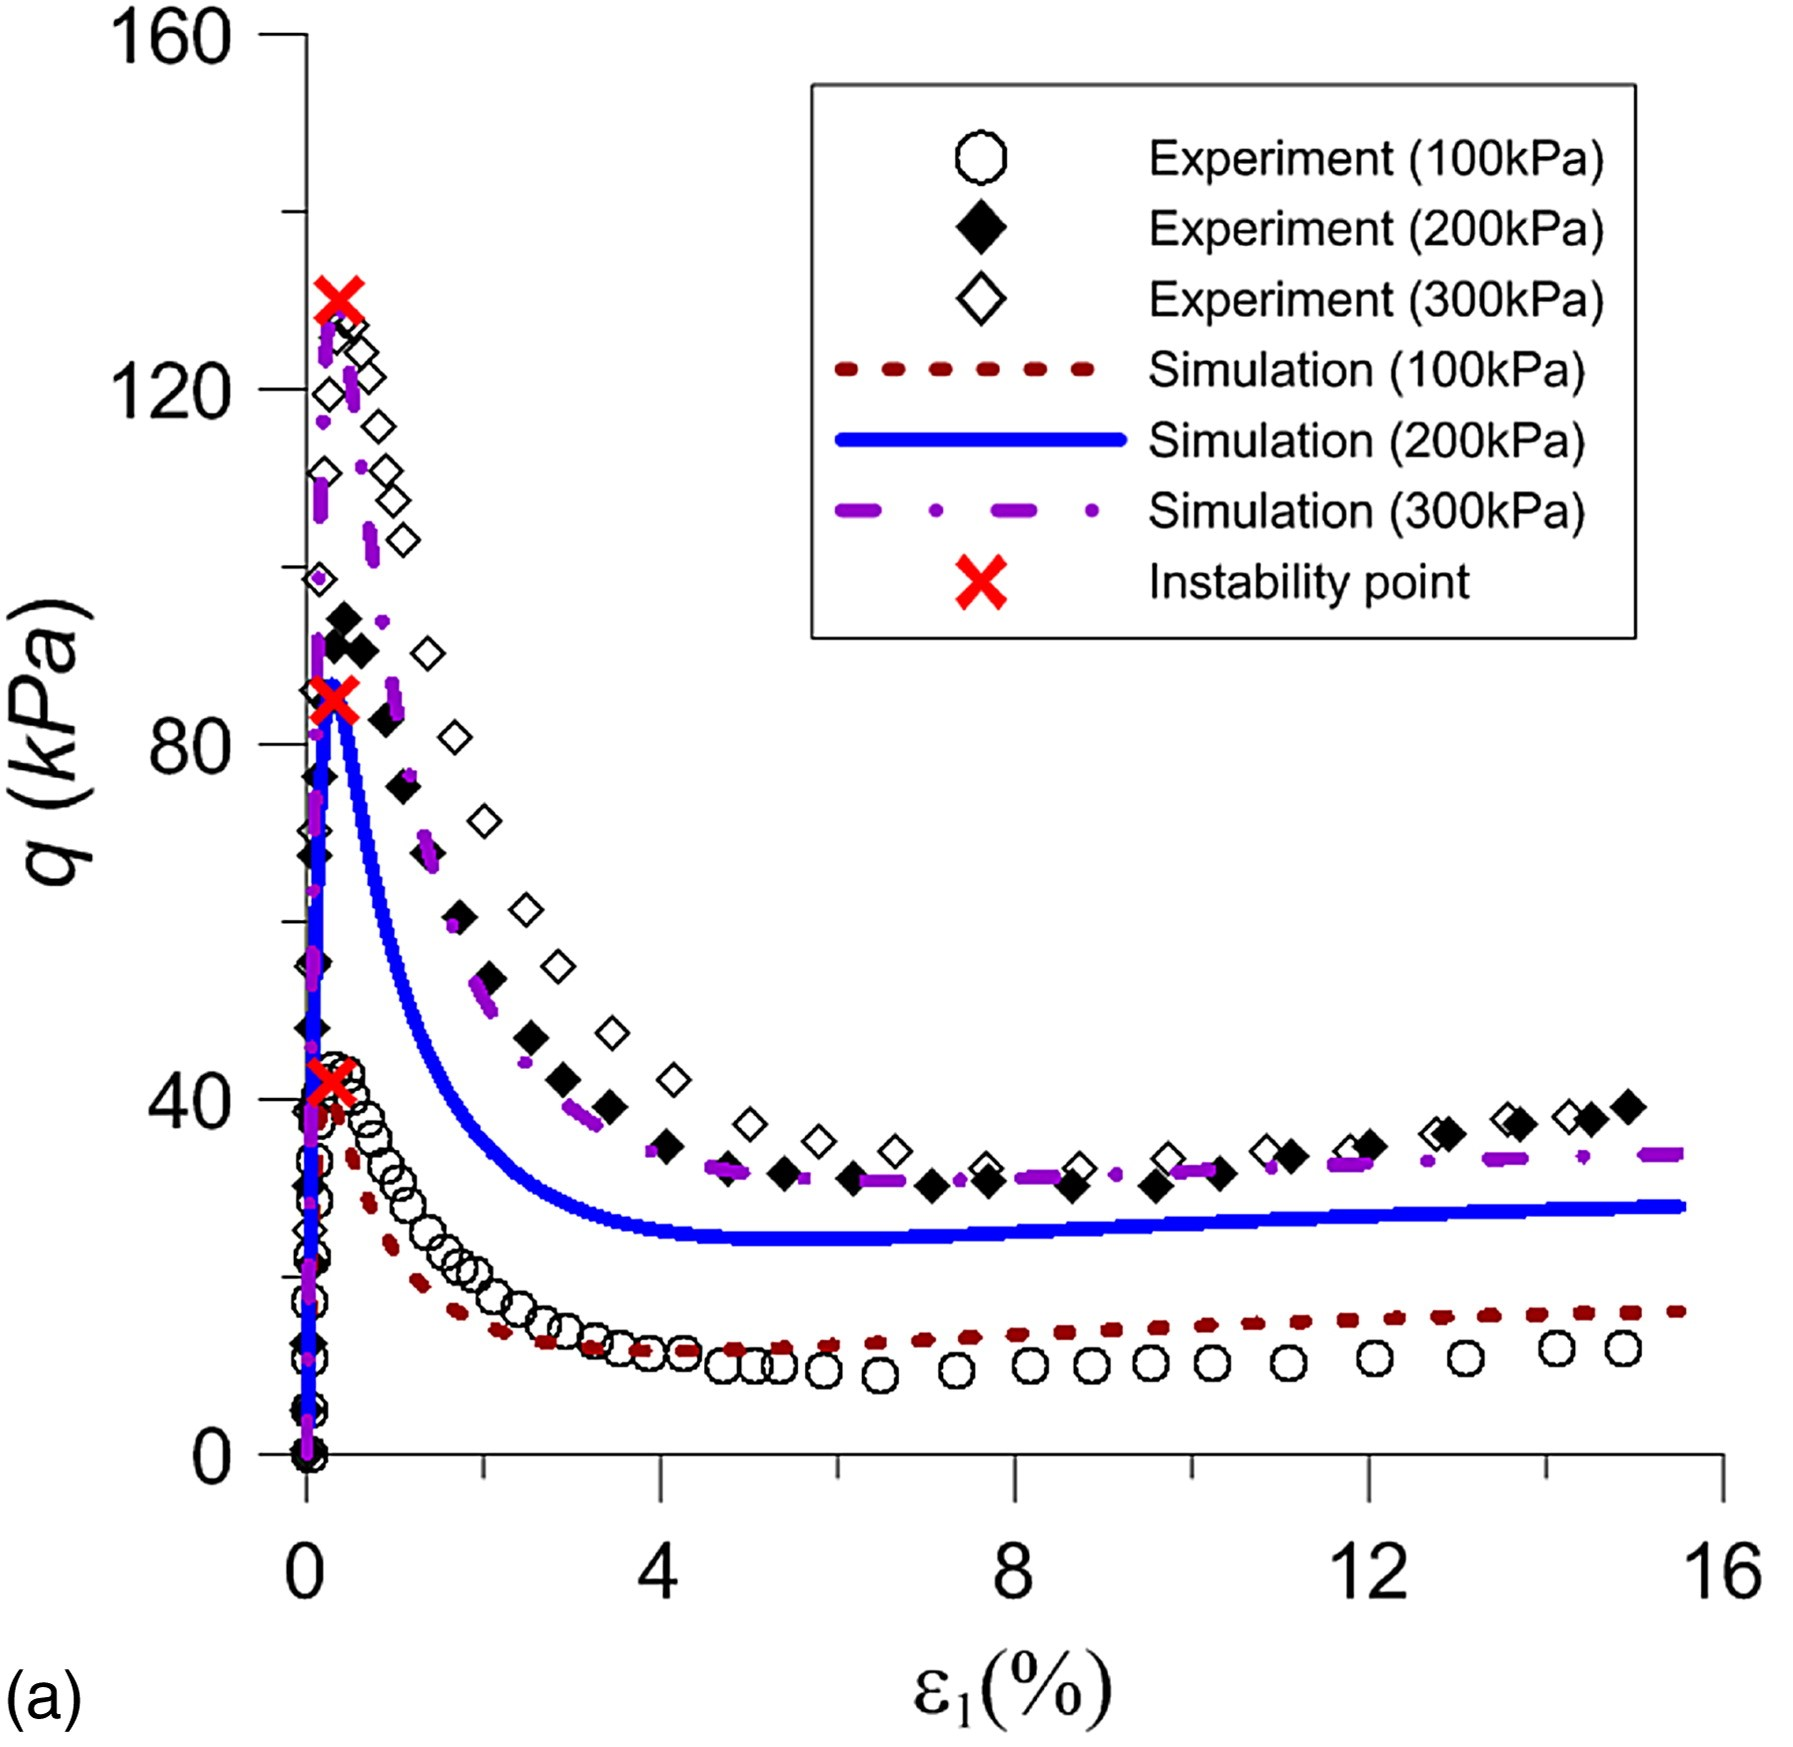
\includegraphics[width=.75\textwidth]{figures/figure5a.jpg}
                \label{figure:5a}
            }
            \subfigure[normalized pore pressure, major principal strain 归一化孔隙水压力,主应变]{
                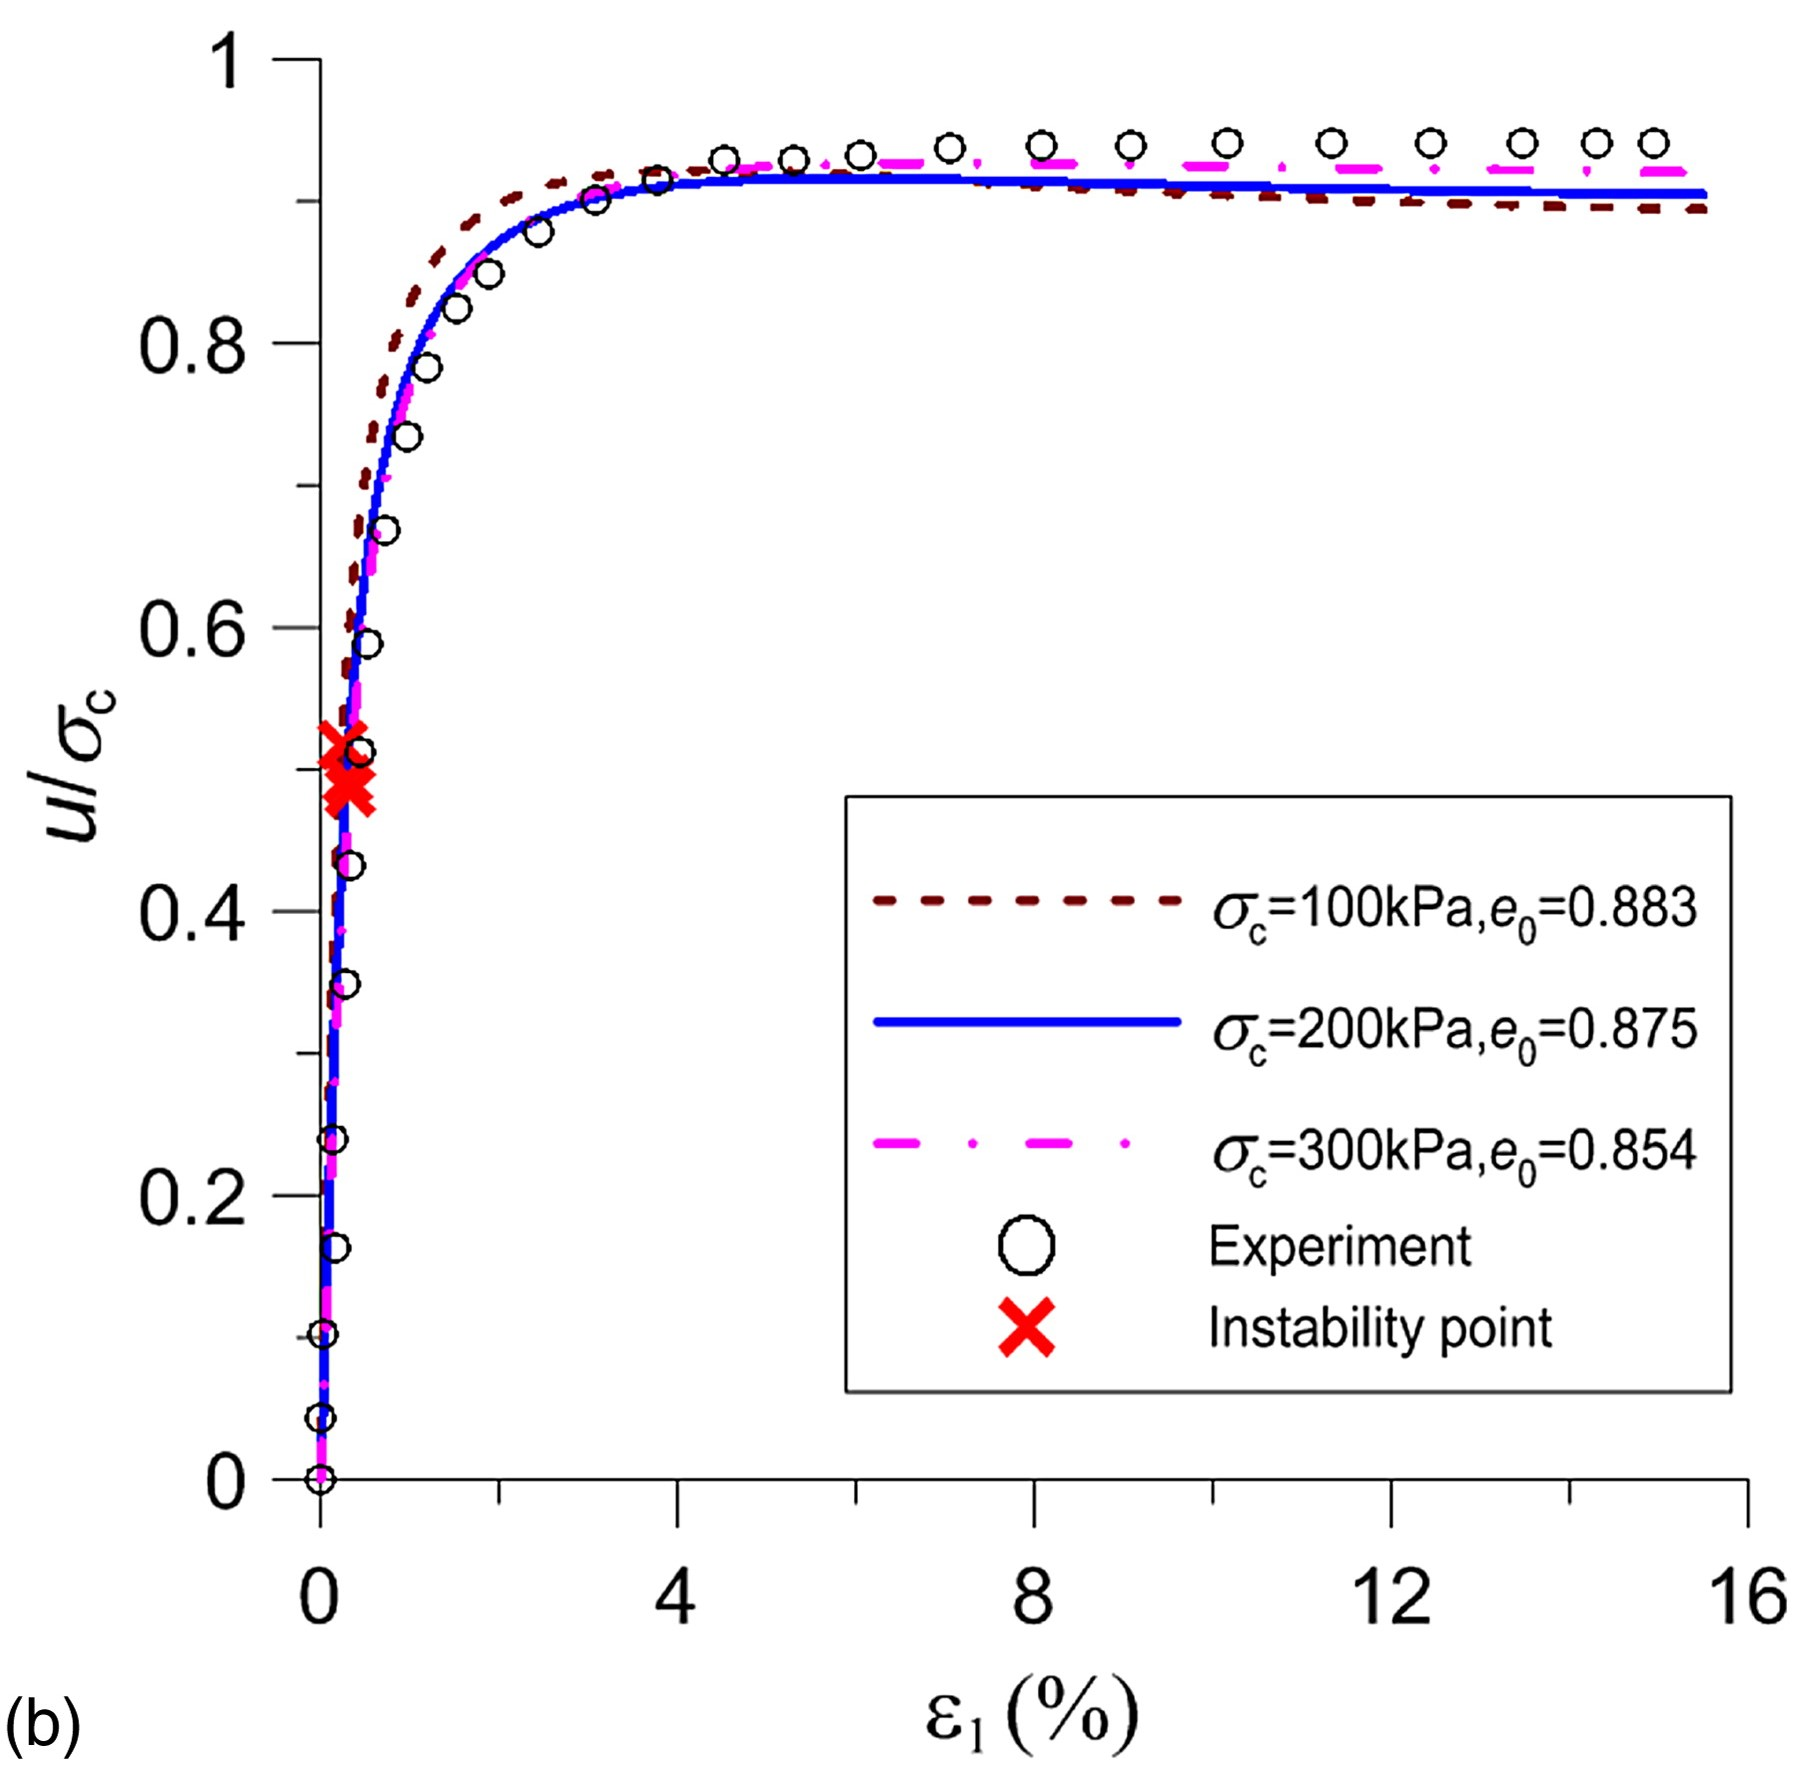
\includegraphics[width=.75\textwidth]{figures/figure5b.jpg}
                \label{figure:5b}
            }
            \bicaption{Model prediction (experimental data from \citealt{Doanh1997})}{模型预测(实验数据来自\citealt{Doanh1997})}
            \label{figure:5}
        \end{figure}
        \begin{figure}[H]
            \centering
            \addtocounter{figure}{1}
            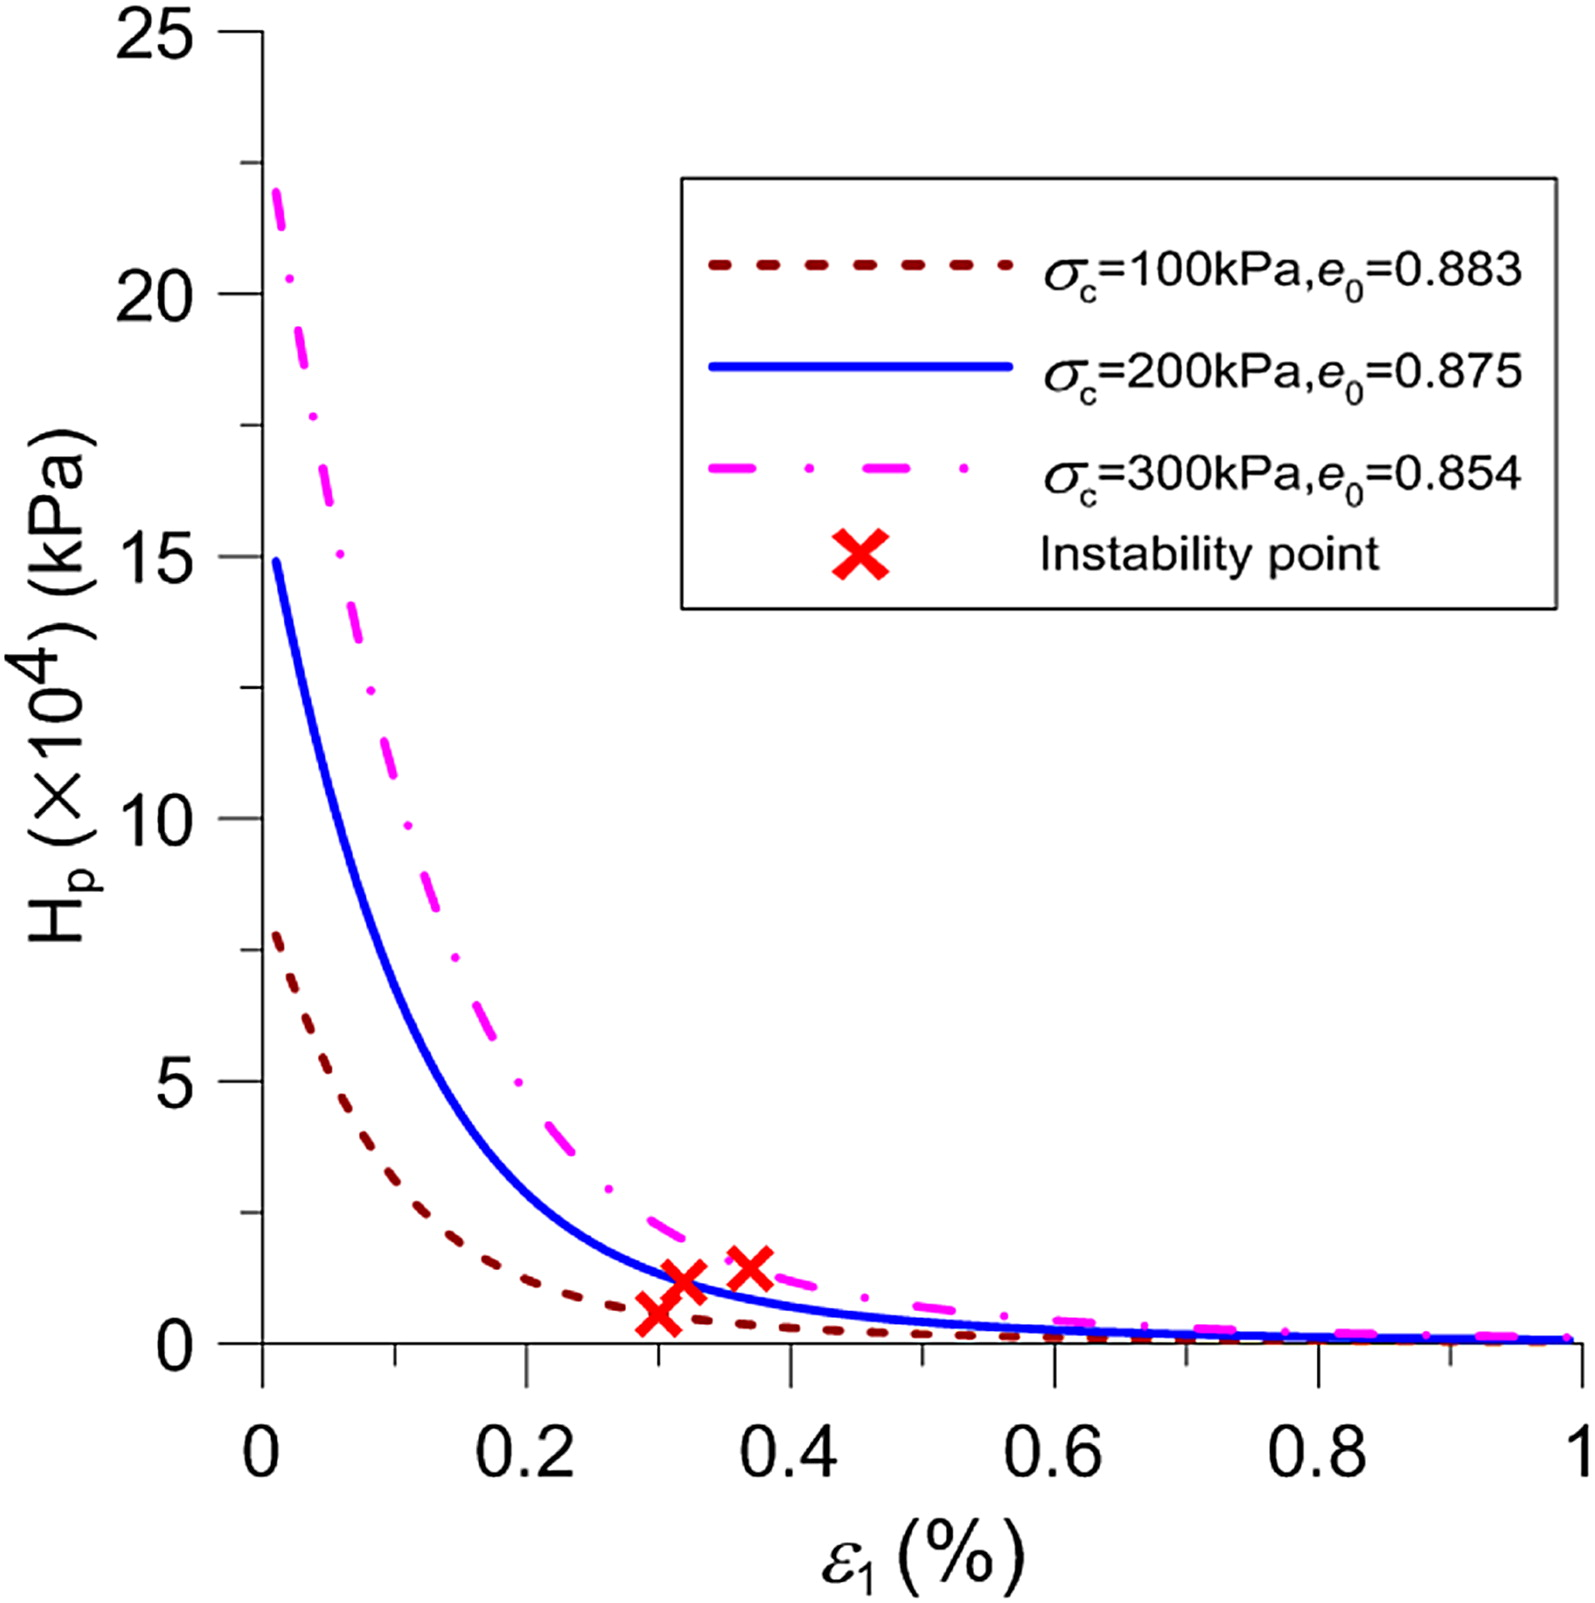
\includegraphics[width=.75\textwidth]{figures/figure7.jpg}
            \bicaption{Evolution of hardening modulus}{硬化模量的演变}
            \label{figure:7}
        \end{figure}
    \end{minipage}
\end{figure}
        \begin{figure}[p]
    \centering
    \begin{minipage}[b]{.48\textwidth}
        \begin{figure}[H]
            \centering
            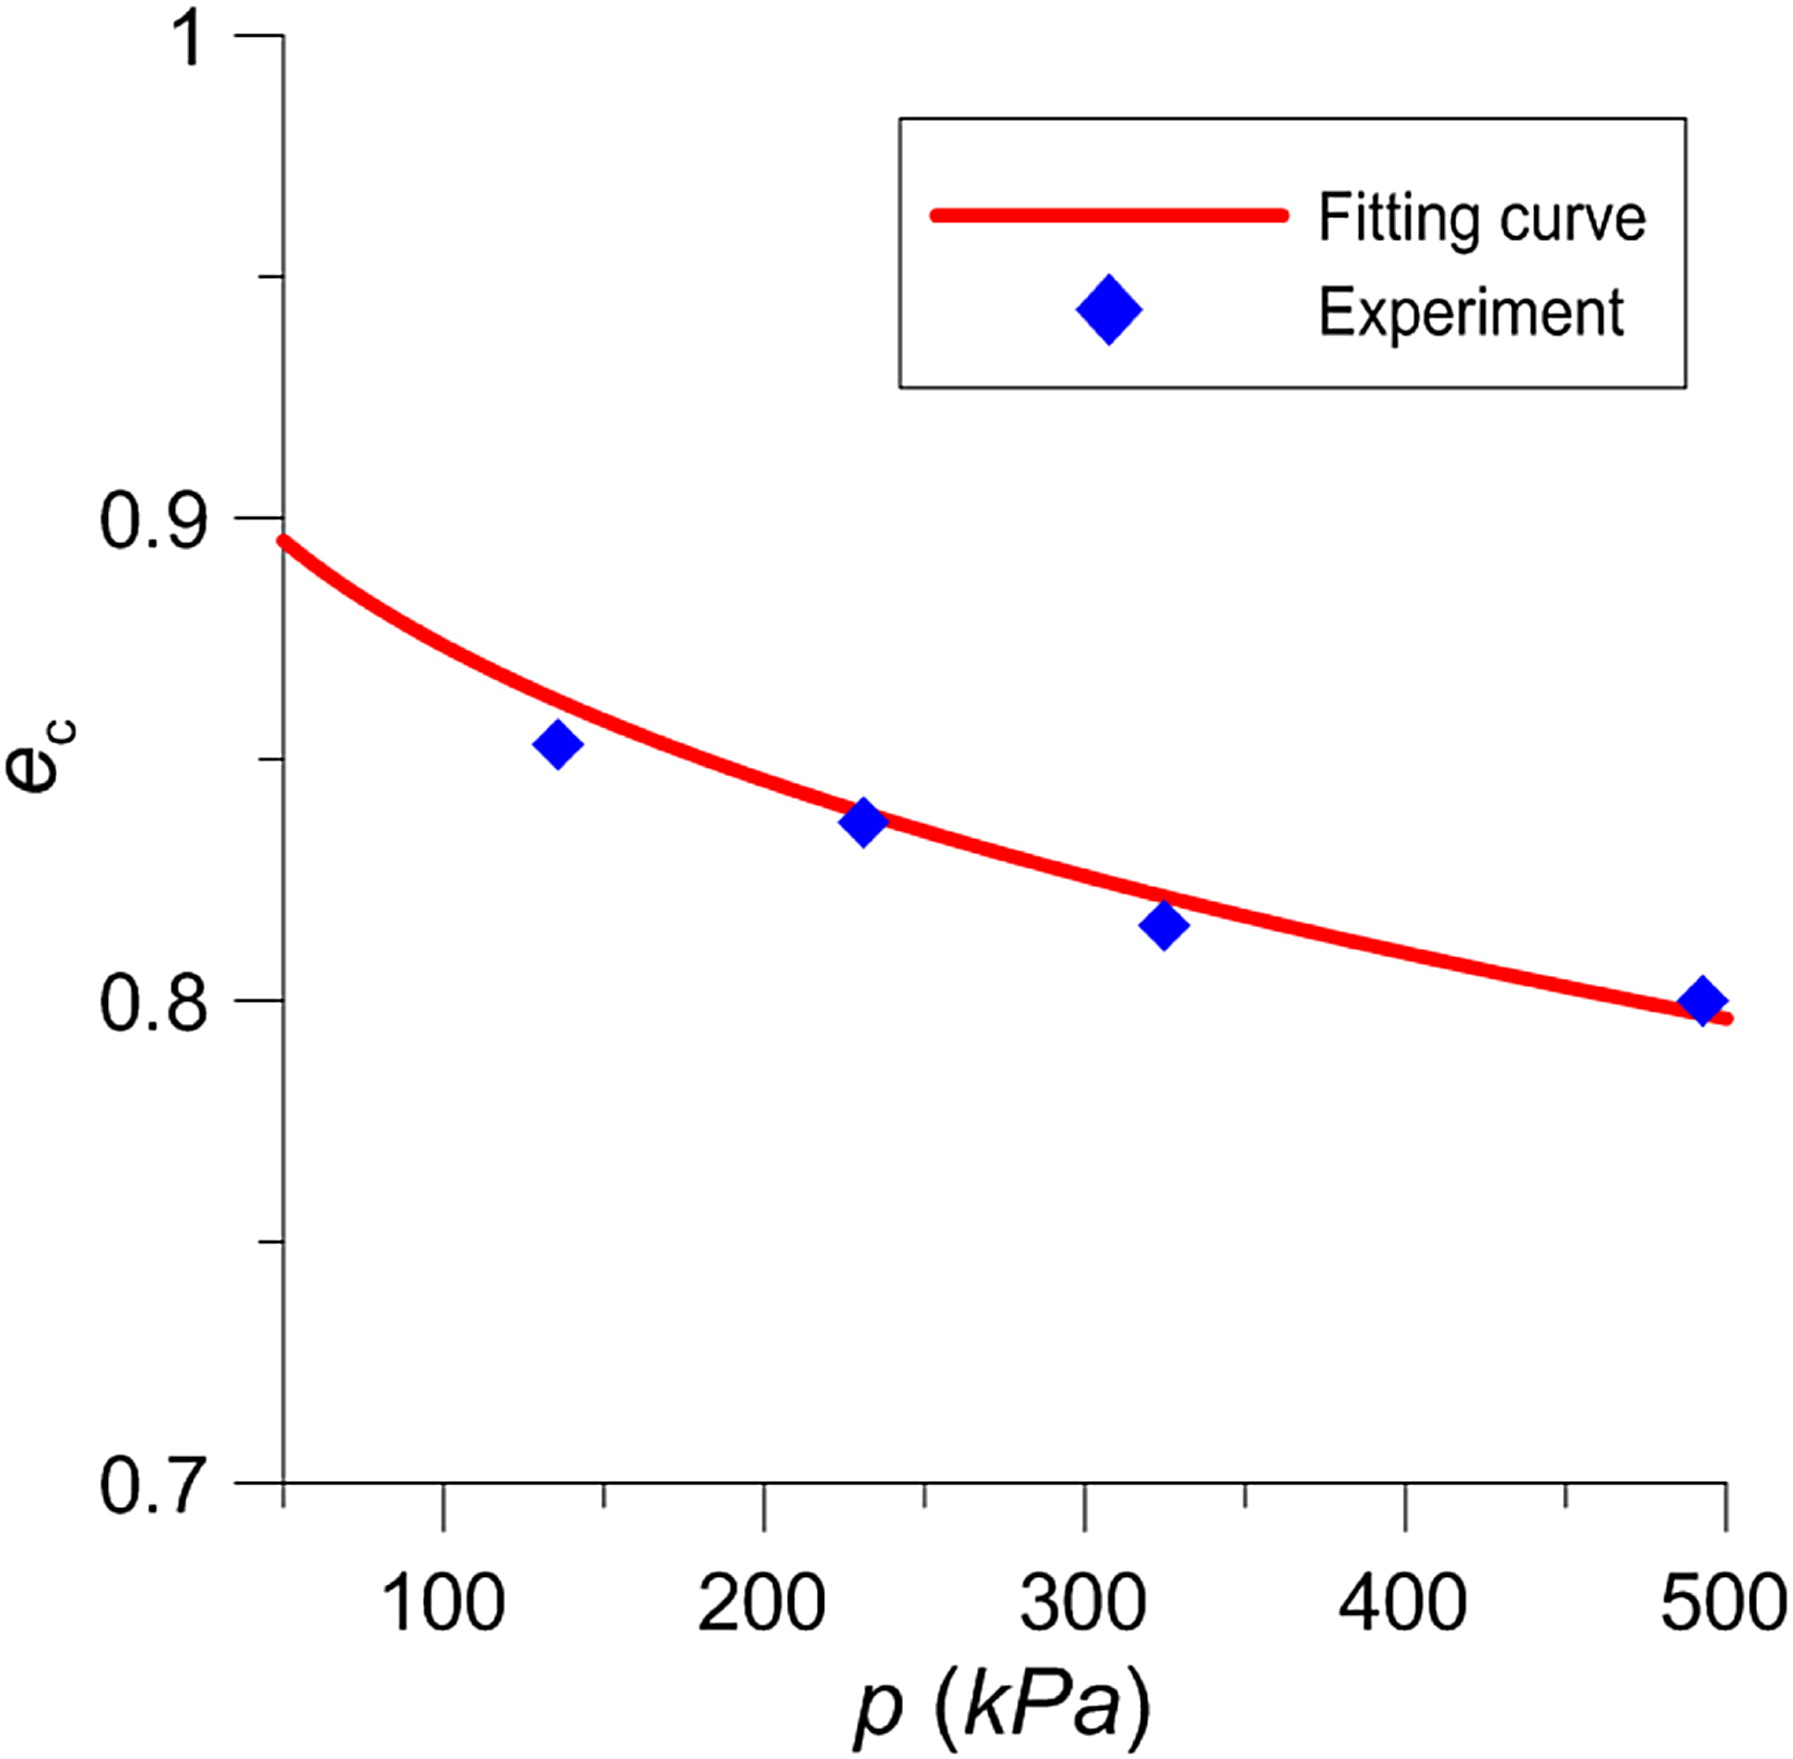
\includegraphics[width=.8\textwidth]{figures/figure8.jpg}
            \bicaption{The $e_c-p$ curve at critical state (experimental data from \citet{Chu2003})}{临界状态下的$e_c-p$曲线(实验数据来自\citealt{Chu2003})}
            \label{figure:8}
        \end{figure}
        \begin{figure}[H]
            \centering
            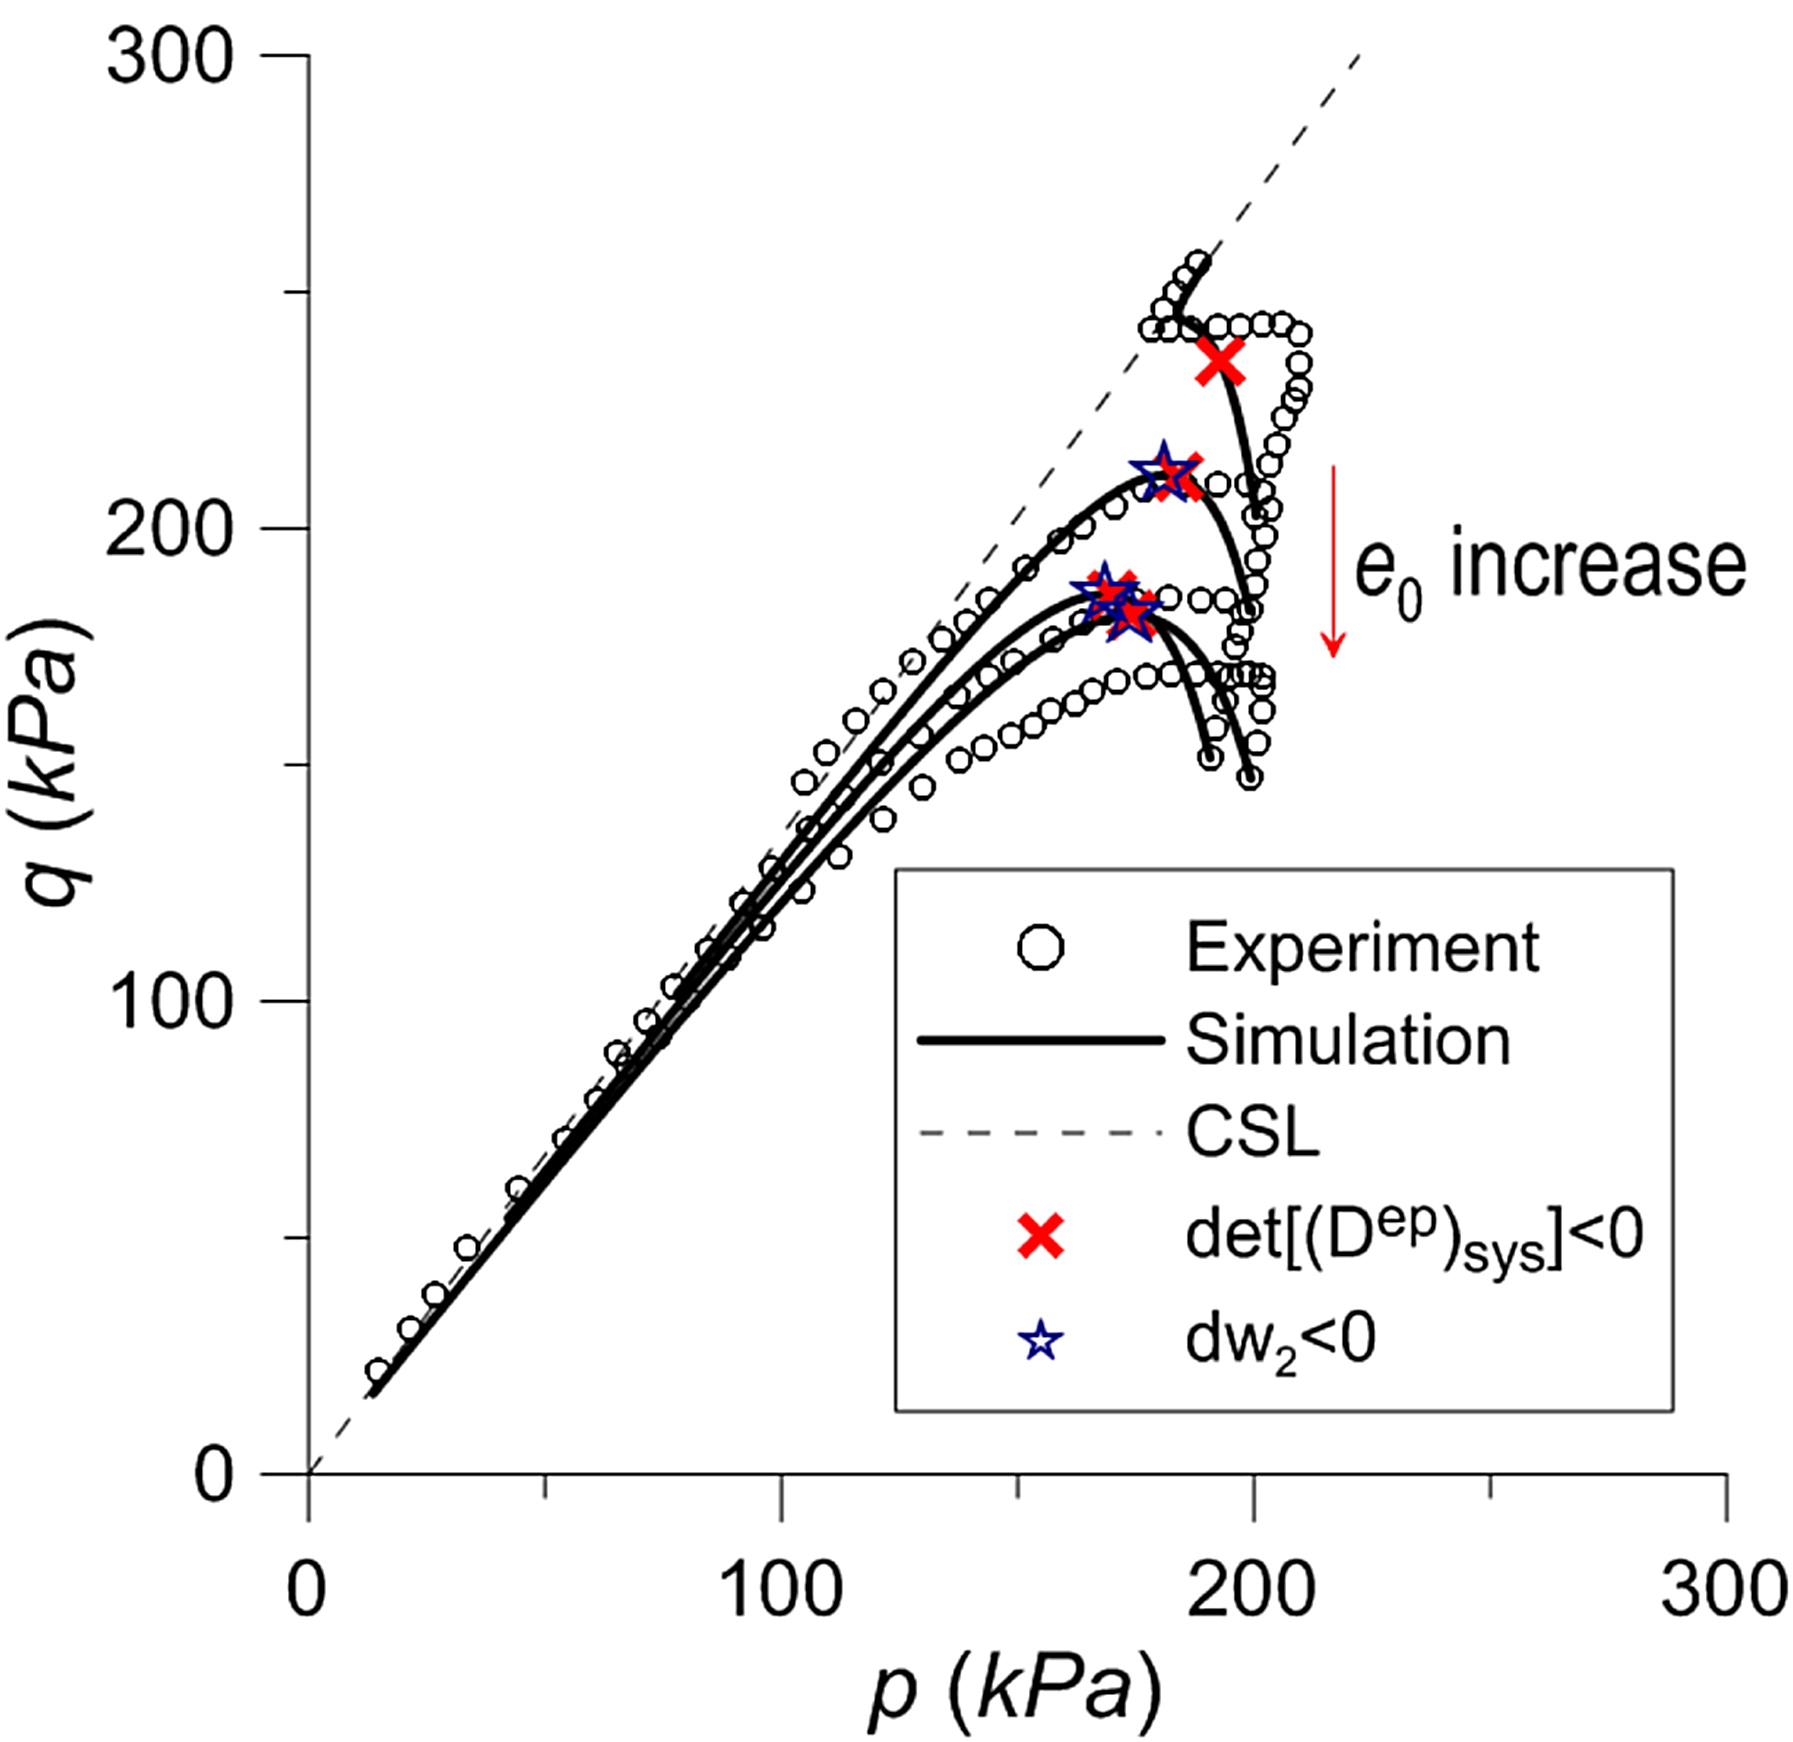
\includegraphics[width=.8\textwidth]{figures/figure9.jpg}
            \bicaption{Stress path of  $K_0$-consolidated undrained triaxial test (experimental data from \citealt{Chu2008})}{$K_0$固结三轴不排水试验的应力路径(实验数据来自\citealt{Chu2008})}
            \label{figure:9}
        \end{figure}
    \end{minipage}
    \hspace{0.02\textwidth}
    \begin{minipage}[b]{.48\textwidth}
        \begin{figure}[H]
            \centering
            \subfigure[stress-strain relationship 应力应变关系]{
                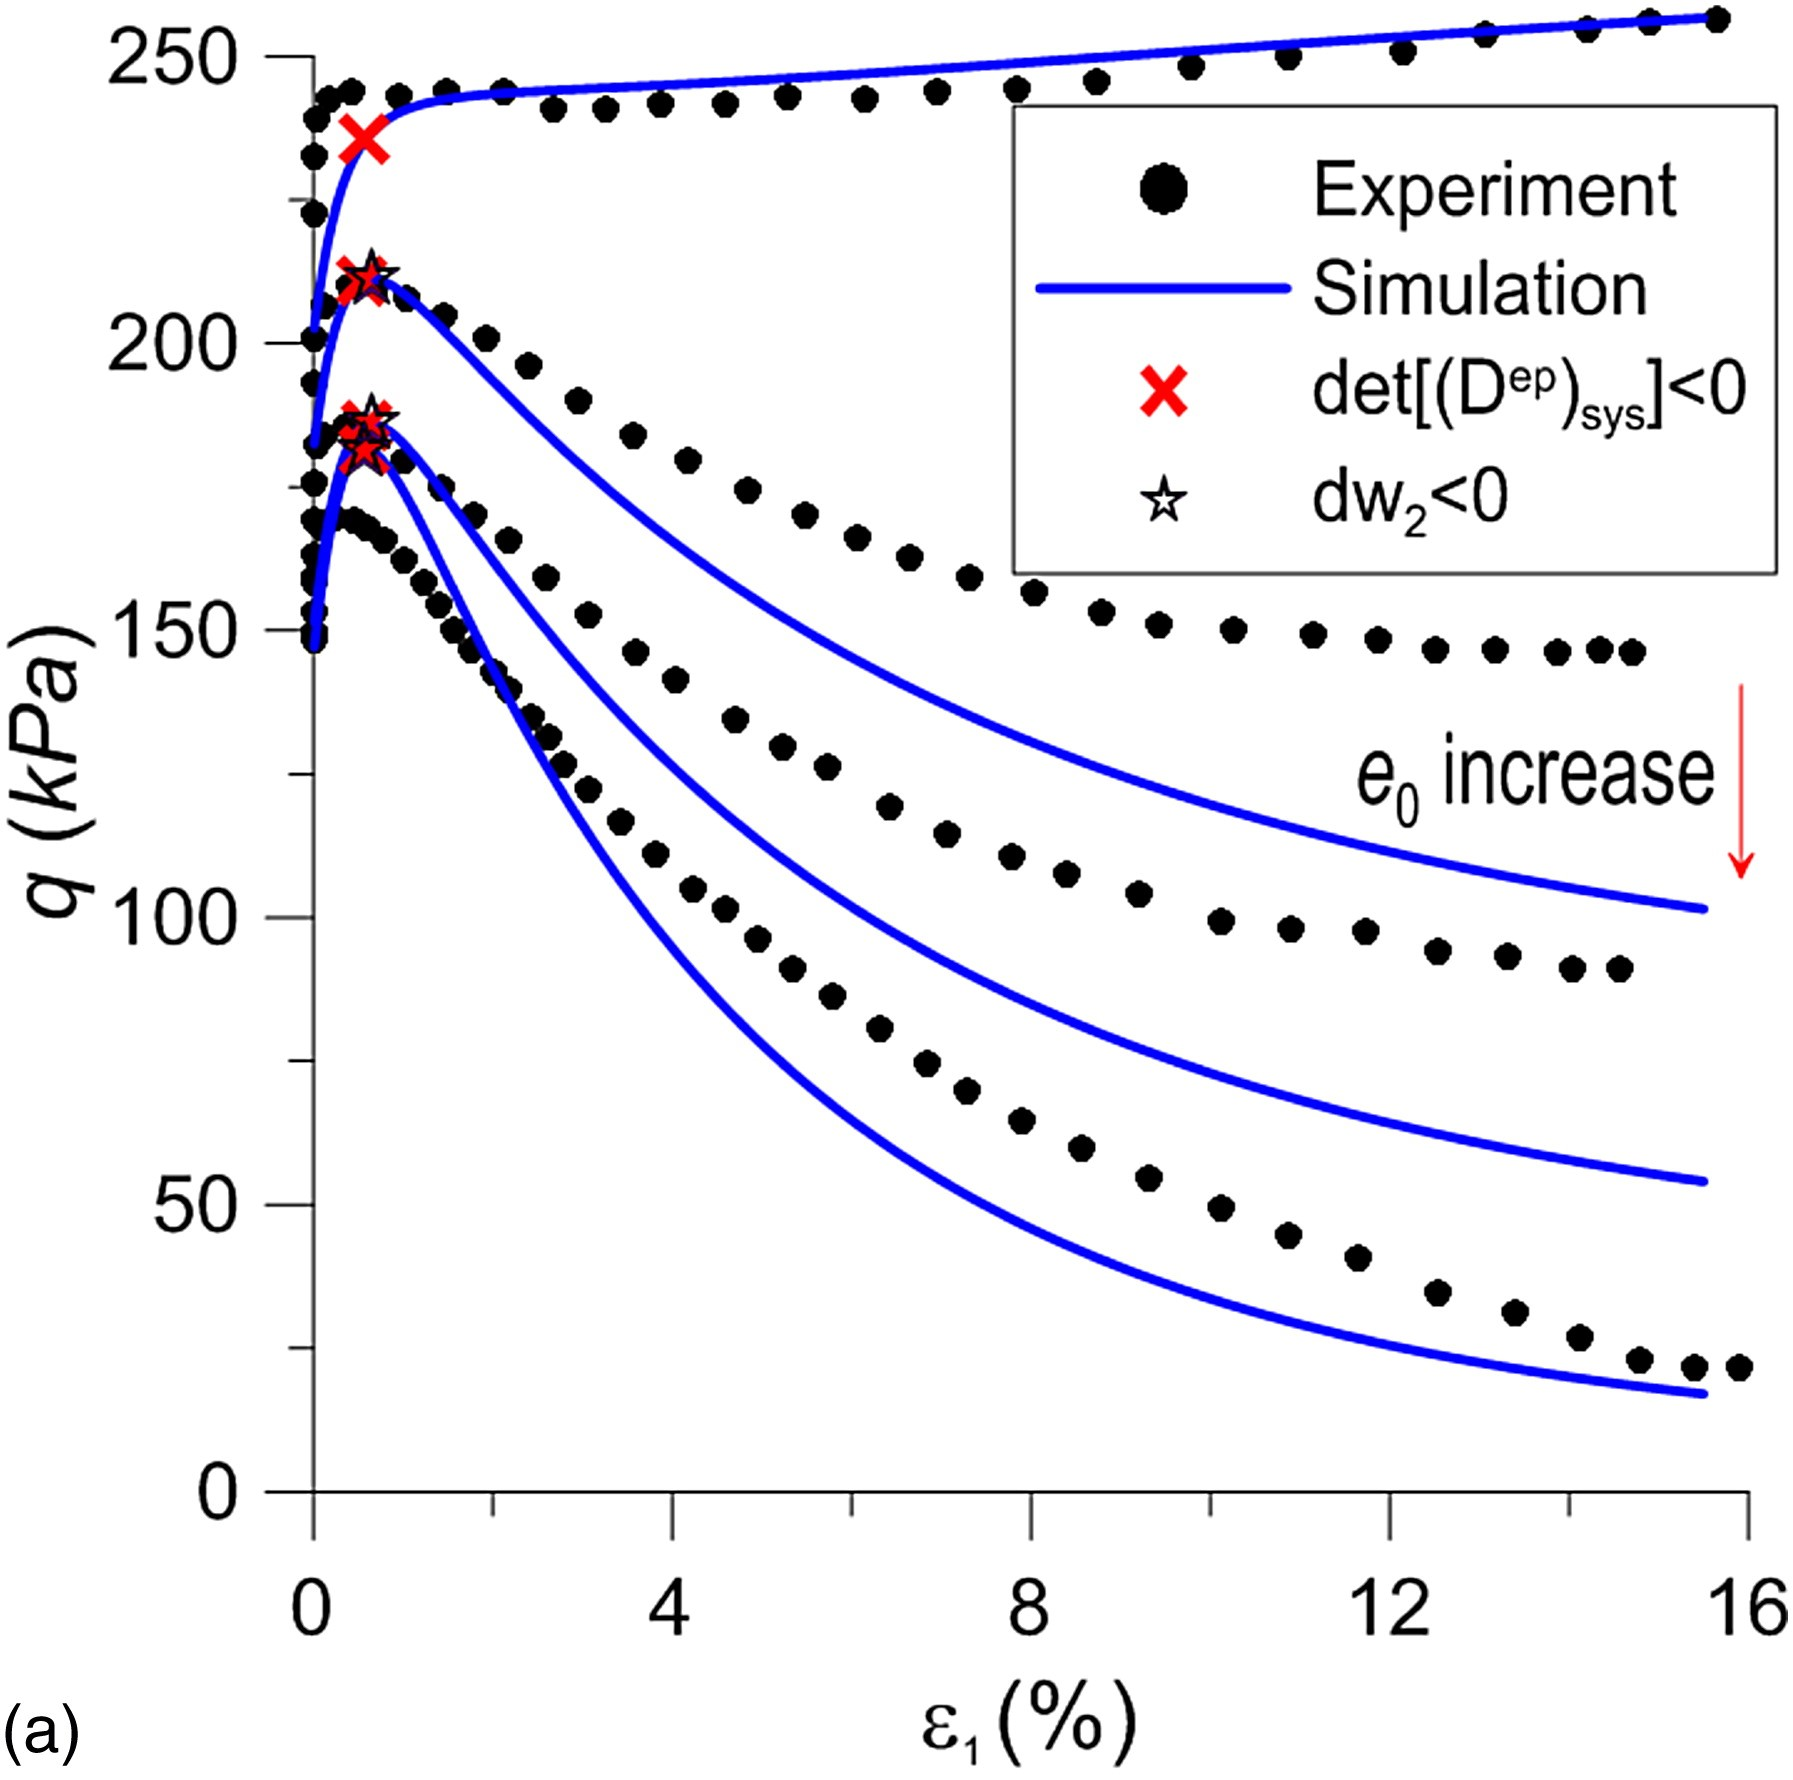
\includegraphics[width=.8\textwidth]{figures/figure10a.jpg}
                \label{figure:10a}
            }
            \subfigure[evolution of pore-water pressure 孔隙水压力的演变]{
                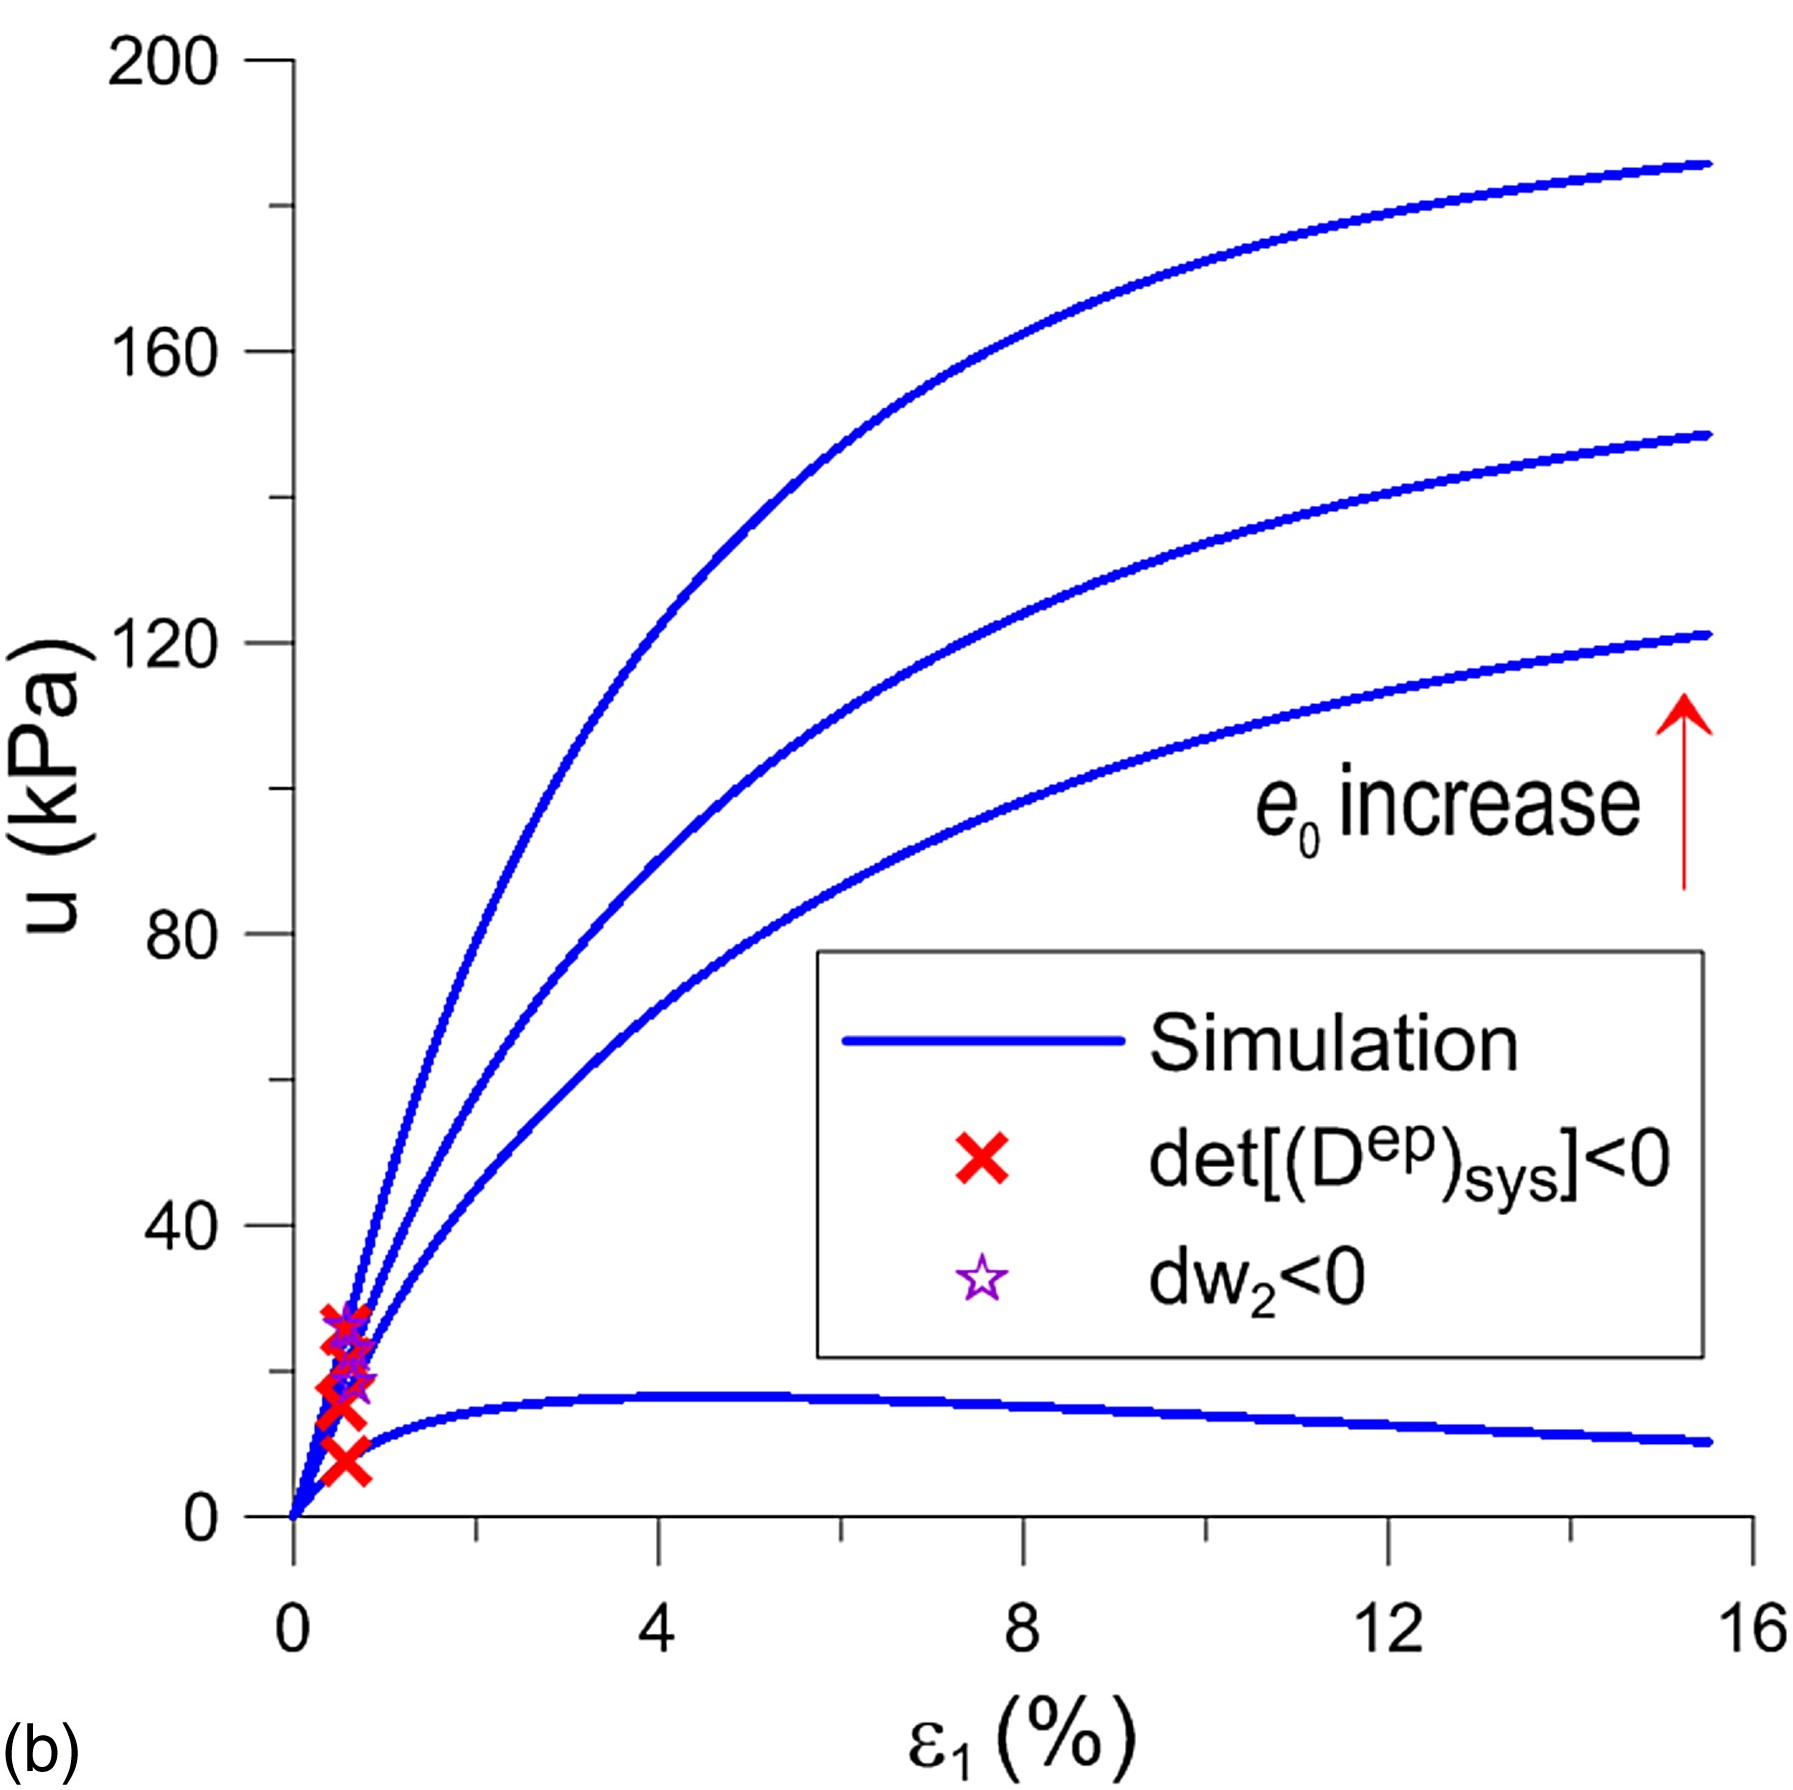
\includegraphics[width=.8\textwidth]{figures/figure10b.jpg}
                \label{figure:10b}
            }
            \bicaption{Model prediction (experimental data after Chu and \citealt{Chu2008})}{模型预测(来自\citealt{Chu2008}之后的实验数据)}
            \label{figure:10}
        \end{figure}
    \end{minipage}
\end{figure}
    }
    \switchcolumn*[\bisubsection*{$K_0$-Consolidated Undrained Triaxial Tests}{$K_0$三轴固结不排水试验}]

    The proposed constitutive model and instability criteria were used to predict the results of the $K_0$-consolidated undrained triaxial tests of \citet{Chu2008}. The specimen was made of Singapore marine-dredged silica sand with mean grain size 0.30–0.35 mm, uniformity coefficient 2.0, specific gravity 2.6, maximum void ratio 0.916, and minimum void ratio 0.533. The specimen was 100 mm in diameter and 190 mm in height. After $K_0$ consolidation, the void ratios of the specimens were 0.844, 0.881, 0.899, and 0.922.

    \switchcolumn

    所提出的本构模型和不稳定性标准被用于预测\citet{Chu2008}的$K_0$三轴固结不排水试验的结果。 样品由新加坡海洋挖出的硅砂制成,平均粒度为0.30–0.35毫米,不均匀系数为2.0,比重为2.6,最大孔隙比为0.916,最小孔隙比为0.533。 样品的直径为100毫米,高度为190毫米。 $K_0$固结后,样品的孔隙比分别为0.844、0.881、0.899和0.922。

    \switchcolumn*

    As shown in \enautoref{figure:8}, the $e_c-p$ curve at the critical state was calibrated from the experimental results of \citet{Chu2003} in the same sands. By using the material parameters in \enautoref{table:1}, the mechanical behavior of the $K_0$-consolidated saturated sands under undrained loading were obtained. The predicted effective stress path is shown in \enautoref{figure:9}. For relatively loose sand ($e_0 = 0.881,0.899,0.922$), the undrained loading induced the reduction of the mean pressure and the increase of deviatoric shear stress; after the attainment of its peak value, the deviatoric shear stress decreased. The test of the densest sands ($e_0 = 0.844$) showed the same trend as with the other three tests at the beginning of the loading stage; when the stress state approached the steady state, the deviatoric shear stress reversed and kept increasing, owing to the phase transition \citep{Ishihara1993}. The predicted stress-strain relationship and pore-water pressure are shown in Figs. \ref{figure:10a} and \ref{figure:10b}. The deviatoric shear stress first increased and then decreased with the applied strain in three relatively loose sand specimens; in the case of the densest sand specimen, the deviatoric shear stress kept increasing and the peak value never appeared. As shown in \enautoref{figure:10b}, the pore-water pressure increased to a constant value when the sands reached the steady state. Compared with the three looser specimens, less pore-water pressure developed in the relatively dense specimen.

    \switchcolumn

    如 \cnautoref{figure:8} 所示,根据 \citet{Chu2003} 在相同砂土中的实验结果,对临界状态下的$e_c-p$曲线进行了校准。通过使用 \cnautoref{table:1} 中的材料参数,获得了在不排水的情况下$K_0$固结的饱和砂土的力学行为。预测的有效应力路径如\cnautoref{figure:9}所示。对于相对疏松的砂土($e_0 = 0.881,0.899,0.922$),不排水的载荷引起平均压力的降低和偏剪应力的增加。达到峰值后,偏剪应力减小。在加载阶段开始时,最稠密的砂的试验($e_0 = 0.844$)显示出与其他三个试验相同的趋势。当应力状态接近稳态时,由于发生了相变,偏剪应力逆转并持续增加 \citep{Ishihara1993}。预测的应力应变关系和孔隙水压力如 \cnautoref{figure:10a} 和 \cnautoref{figure:10b} 所示。在三个相对松散的砂岩样品中,随施加的应变,偏向剪切应力首先增大,然后减小。在最稠密的砂土样品中,偏剪应力不断增加,并且从未出现峰值。如 \cnautoref{figure:10b} 所示,当砂达到稳态时,孔隙水压力增加到一个恒定值。与三个较松散的样品相比,在相对致密的样品中产生的孔隙水压力较小。

    \switchcolumn*

    The determinant of the symmetric part of elastoplastic modulus tensor [\enautoref{figure:11a}] and the second-order work [\enautoref{figure:11b}] were calculated; all the determinants became negative when loading to approximately $0.6\%$ of axial strain, which indicates that all the samples entered into potentially unstable states. As shown in \enautoref{figure:11b}, the second-order work for the densest specimen ($e_0=0.844$) never turned negative, which indicates that static liquefaction would not occur. As shown in \enautoref{figure:12}, although the stresses showed a descending trend after the onset of static liquefaction, both the potentially unstable points and static liquefaction point occurred at the hardening regime. To clarify the influence of the initial material state on the shear strength at static liquefaction, the relationship between the initial void ratio and the stress ratio at the instability point is shown in \enautoref{figure:12}. The stress ratio at the instability point decreased along with the increase of initial void ratio, and the predicted results agreed with the experimental results.

    \switchcolumn

    计算弹塑性模量张量(\cnautoref{figure:11a})的对称部分和二次功(\cnautoref{figure:11b})的行列式;当加载到轴向应变的大约$0.6\%$时,所有决定因素都变为负值,这表明所有样本都进入了潜在的不稳定状态。如\cnautoref{figure:11b}所示,最稠密样品($e_0 = 0.844$)的二阶功从未变为负值,这表明不会发生静态液化。如\cnautoref{figure:12}所示,尽管在静态液化开始后应力显示出下降的趋势,但潜在的不稳定点和静态液化点都发生在硬化区。为了阐明初始材料状态对静态液化时抗剪强度的影响,初始孔隙率与不稳定性点处的应力比之间的关系如\cnautoref{figure:3}所示。不稳定性点处的应力比随着增加而减小初始空隙率的计算结果与实验结果吻合。

    \CrossColumnText{
        \begin{figure}[p]
    \centering
    \begin{minipage}[b]{.48\textwidth}
        \begin{figure}[H]
            \centering
            \subfigure[determinant of the symmetric part of the elastoplastic modulus tensor 弹塑性模量张量的对称部分的行列式的演变]{
                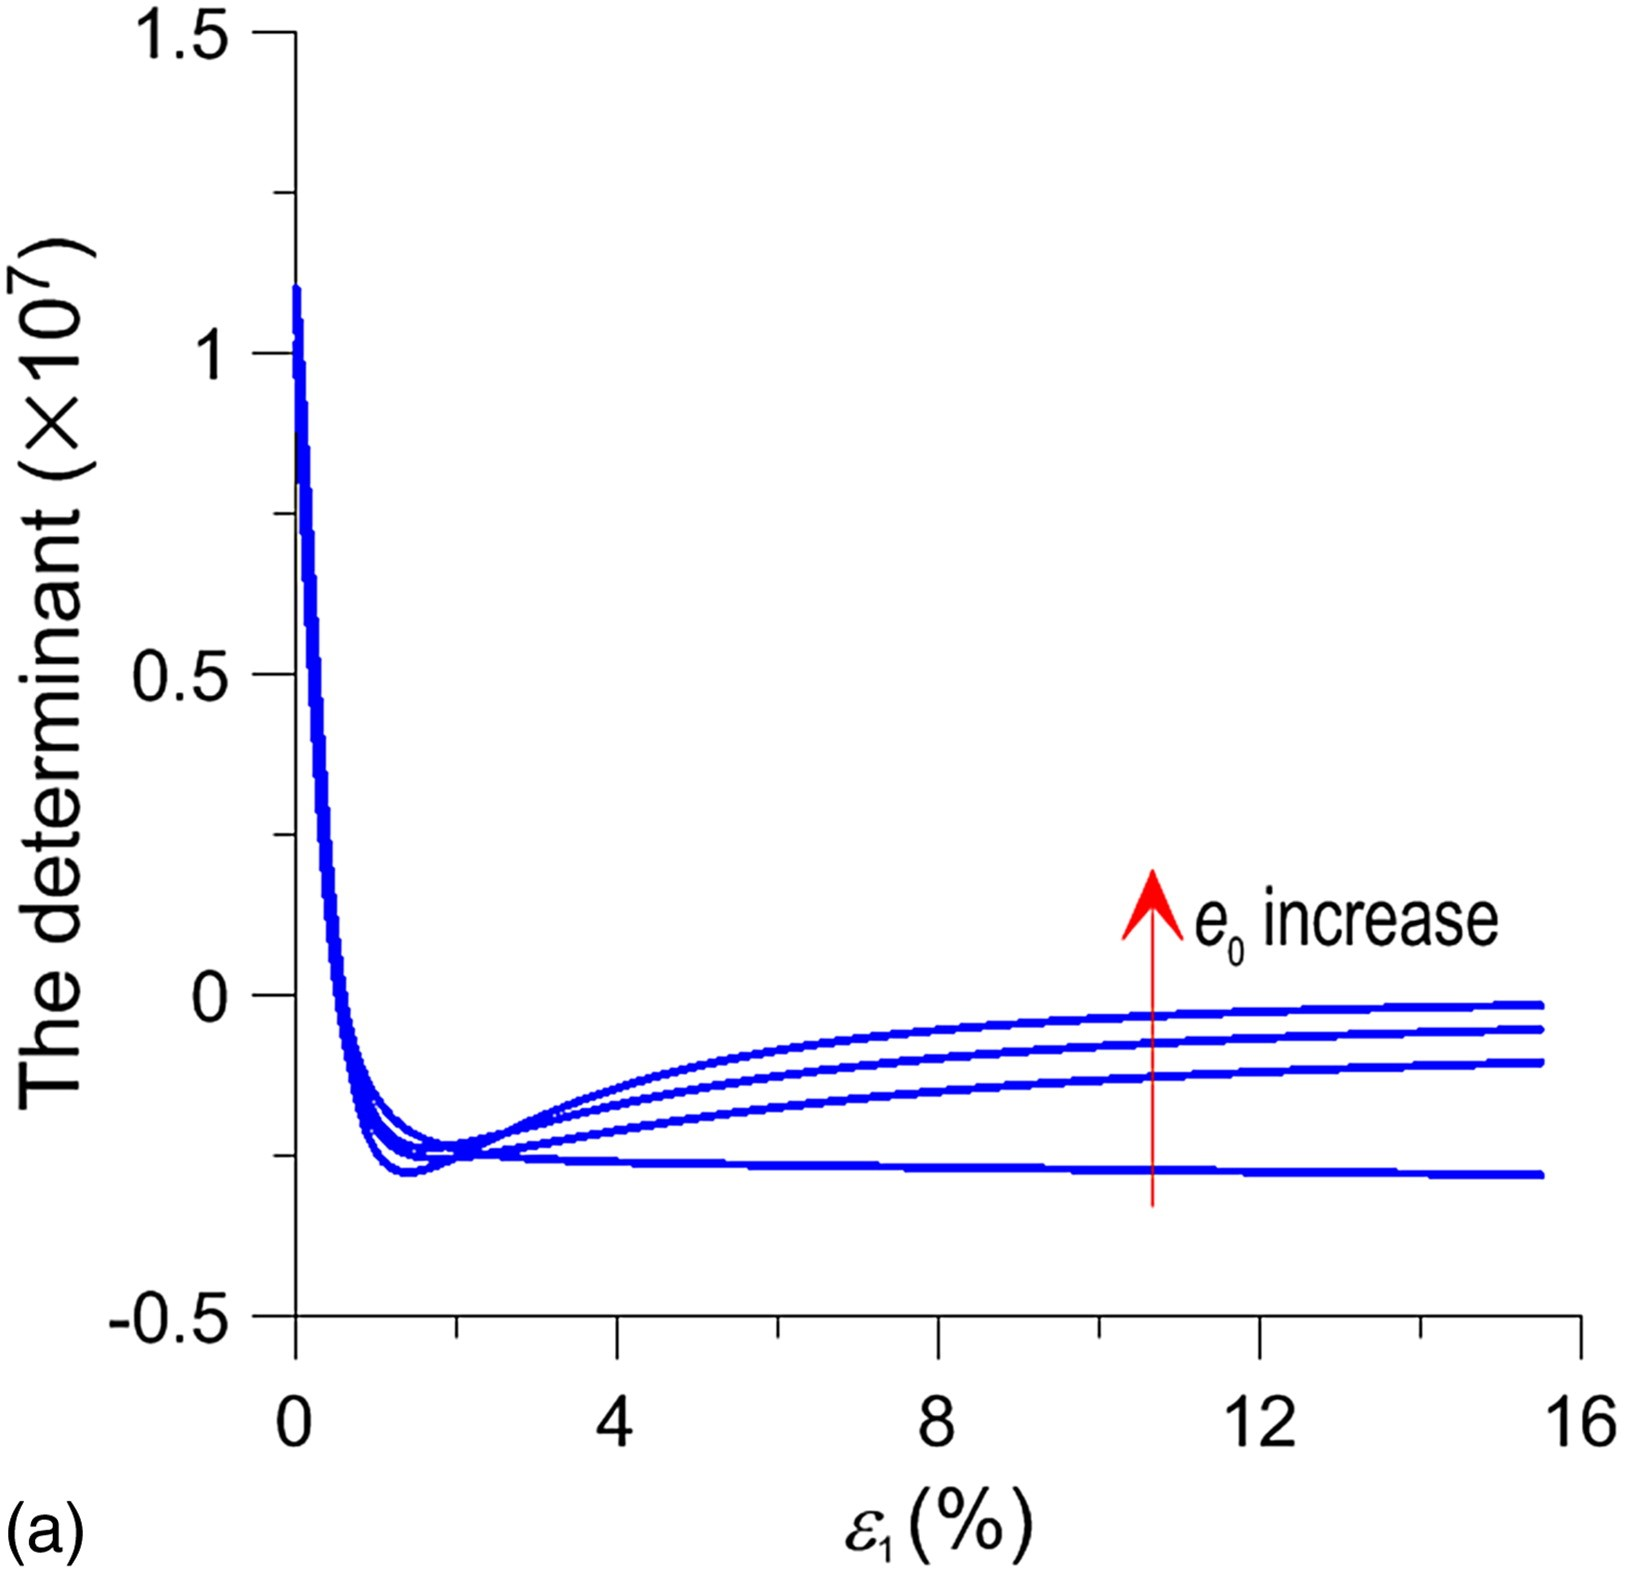
\includegraphics[width=\textwidth]{figures/figure11a.jpg}
                \label{figure:11a}
            }
            \subfigure[evolution of second-order work 二阶功]{
                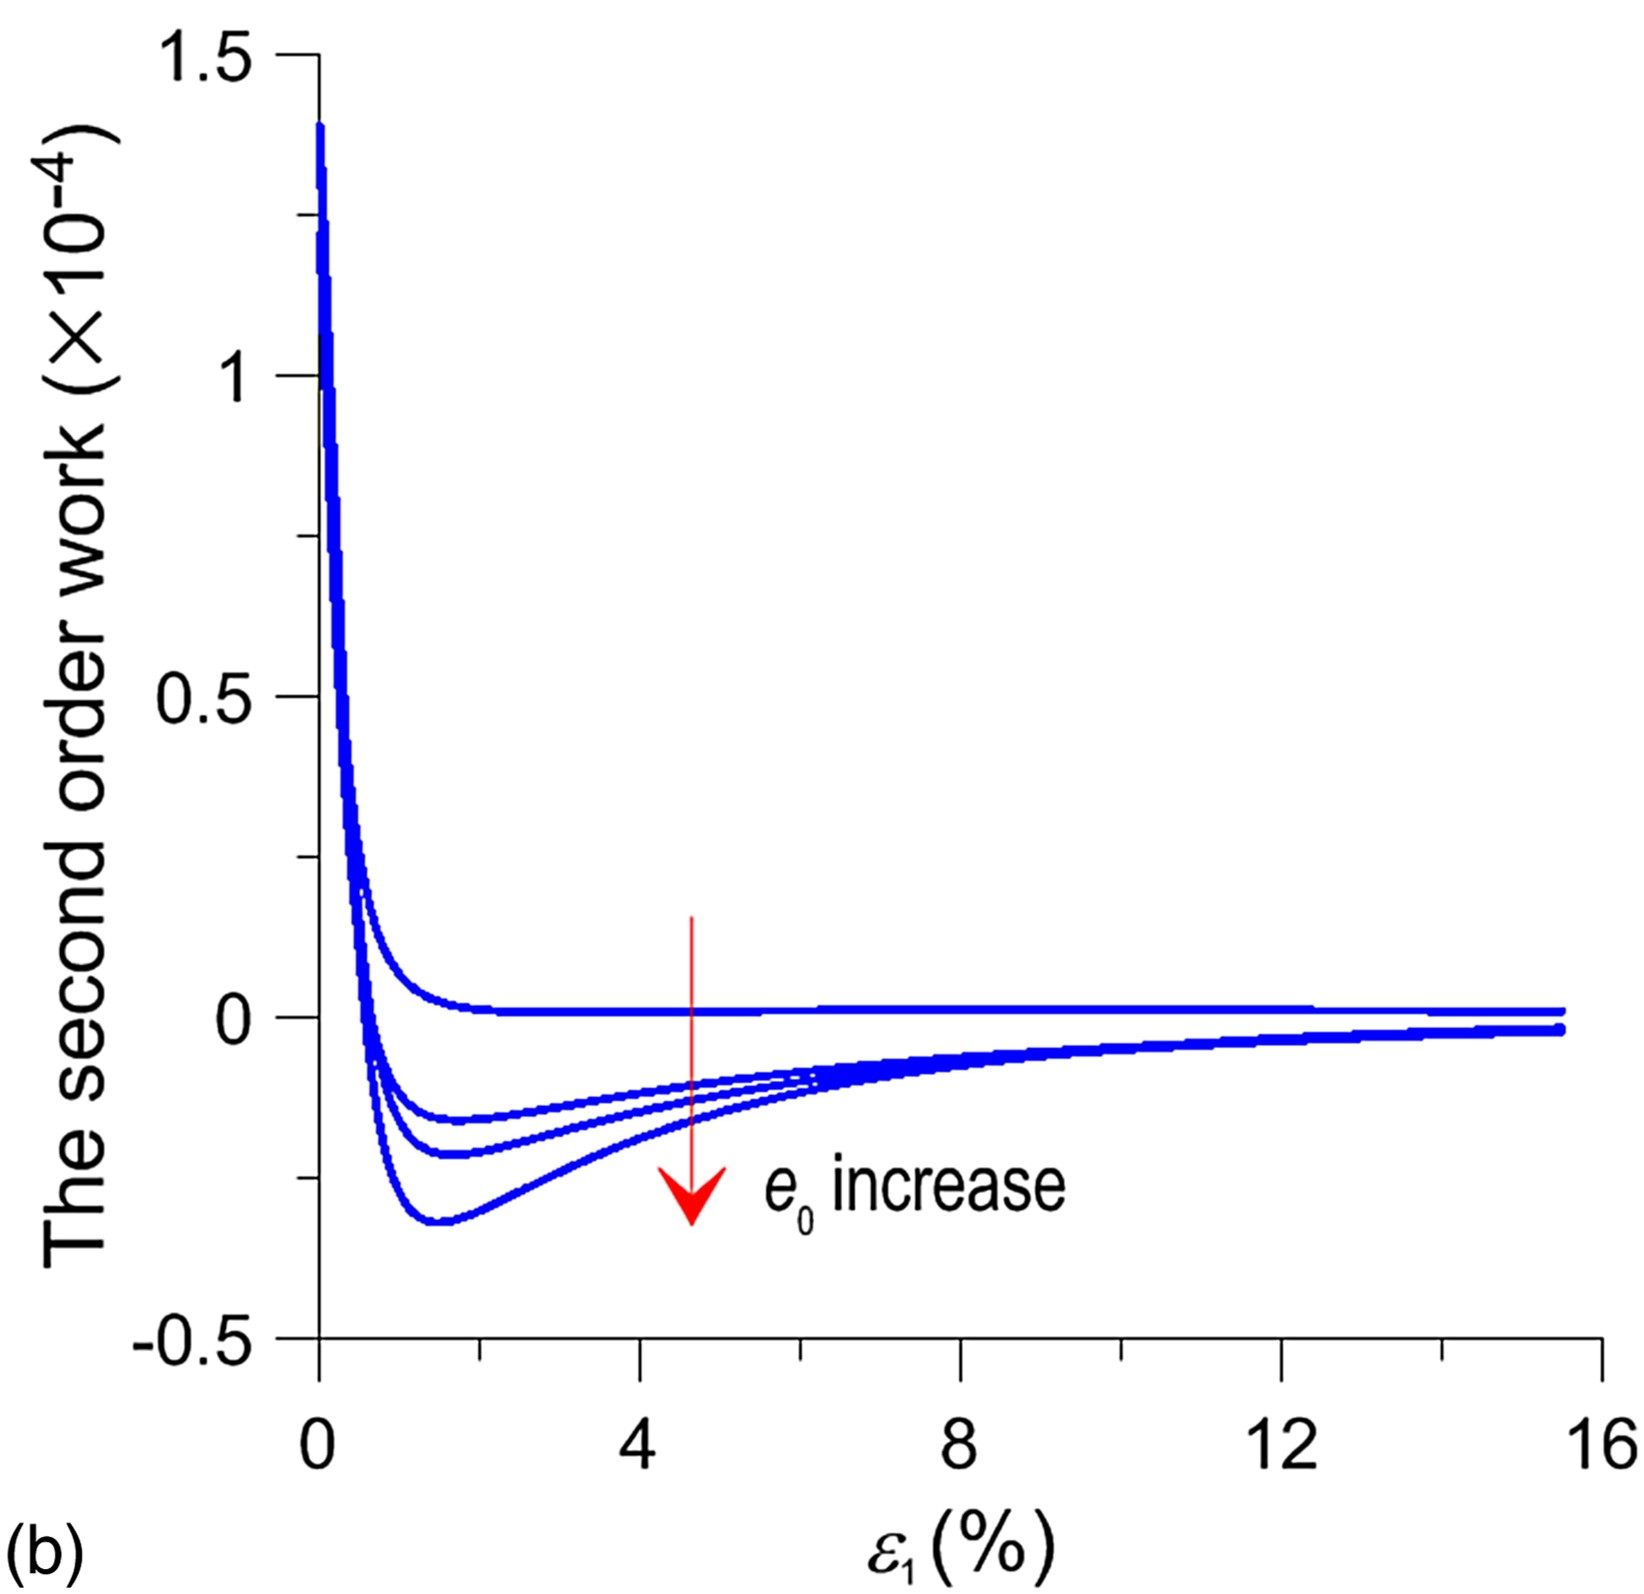
\includegraphics[width=\textwidth]{figures/figure11b.jpg}
                \label{figure:11b}
            }
            \bicaption{Evolution of determinant of the symmetric part of the elastoplastic modulus tensor and second-order work}{弹塑性模量张量的对称部分的行列式的和二阶功的演变}
            \label{figure:11}
        \end{figure}
    \end{minipage}
    \hspace{0.02\textwidth}
    \begin{minipage}[b]{.48\textwidth}
        \begin{figure}[H]
            \centering
            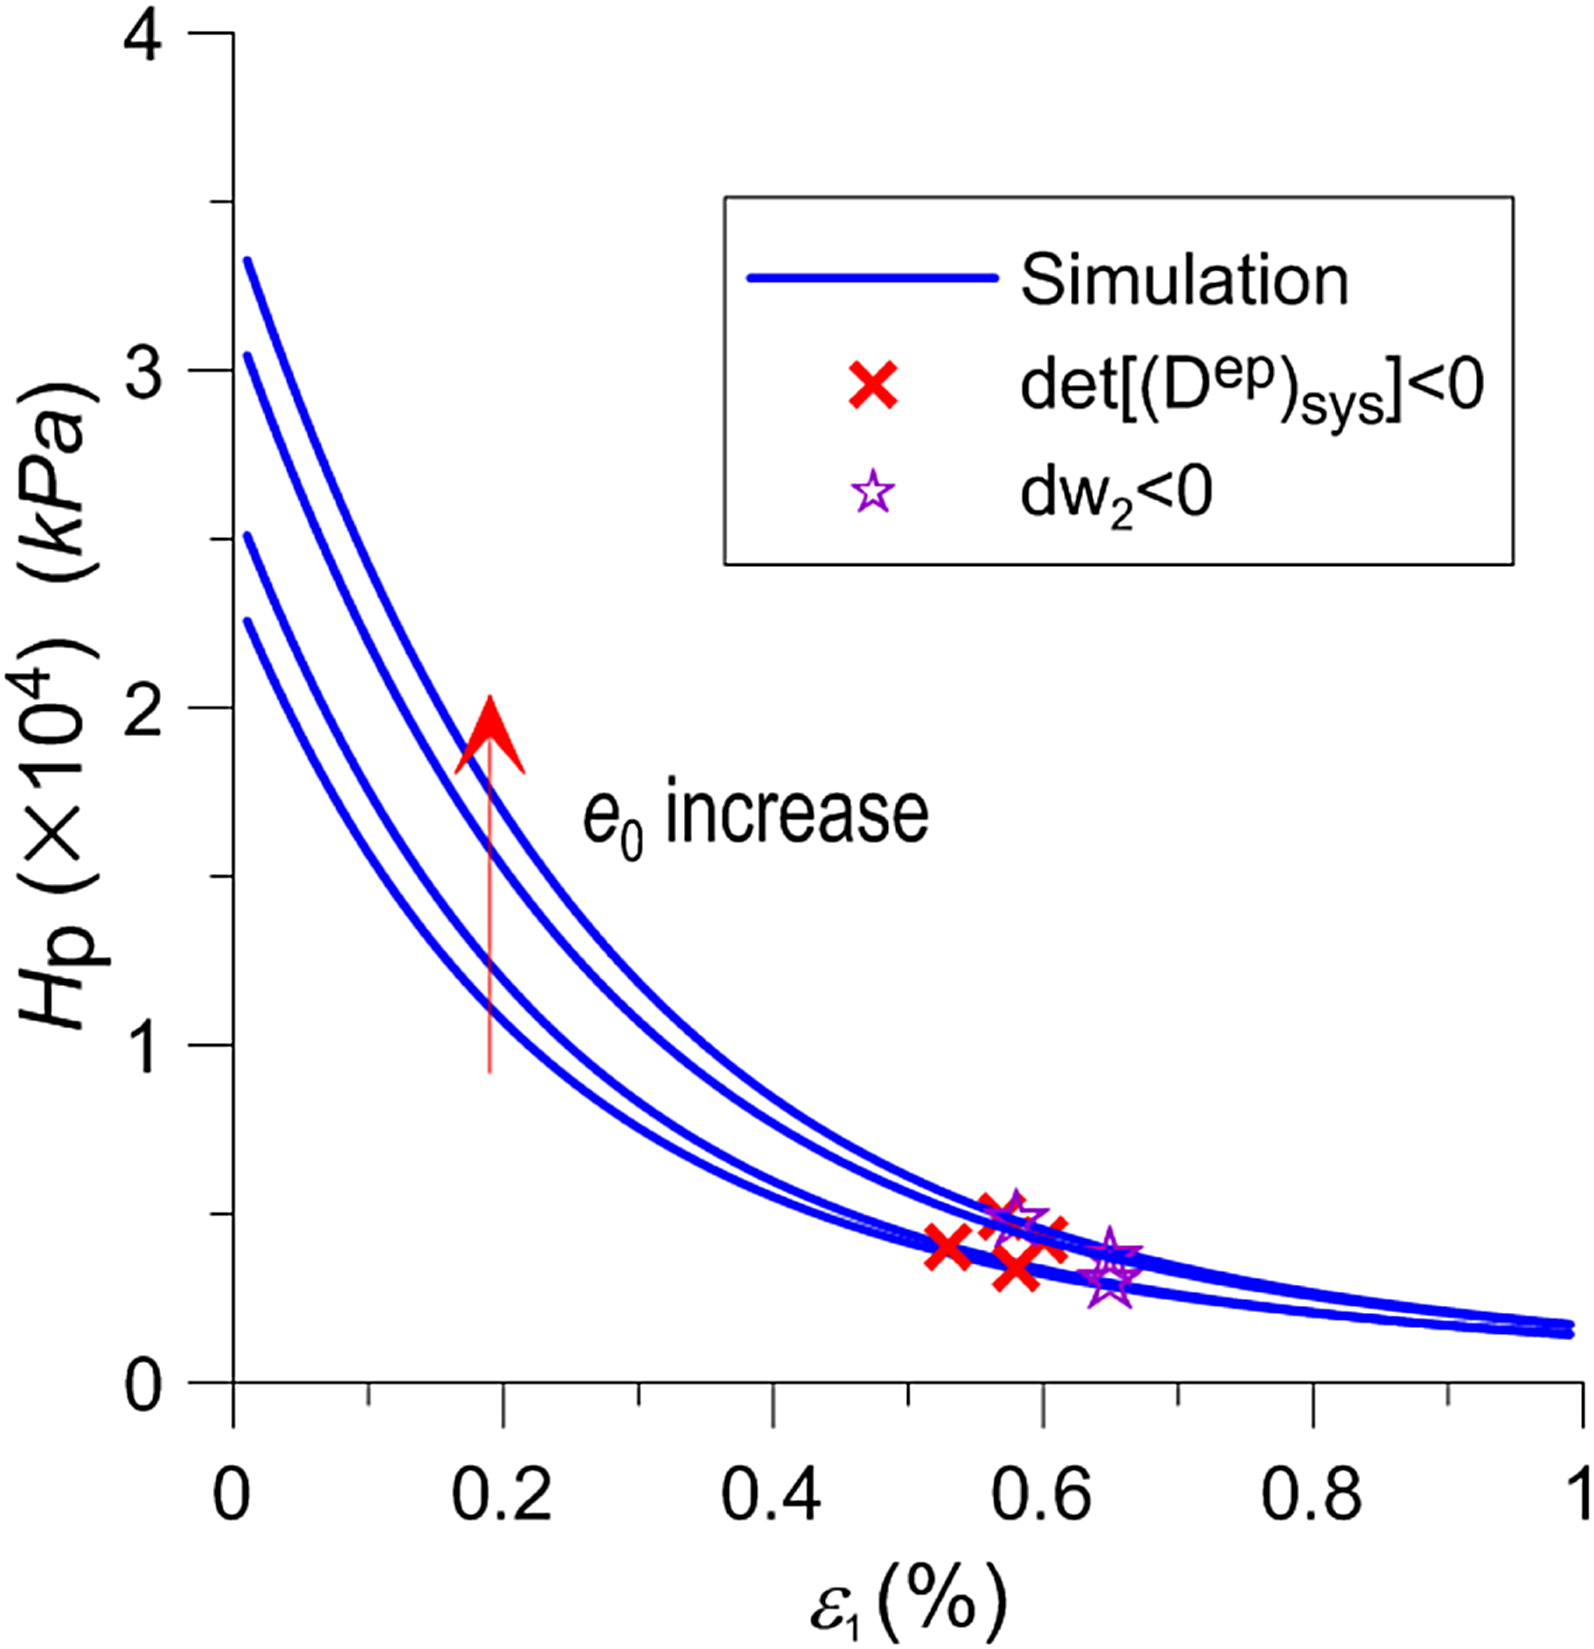
\includegraphics[width=\textwidth]{figures/figure12.jpg}
            \bicaption{Evolution of hardening modulus}{硬化模量的演变}
            \label{figure:12}
        \end{figure}
        \begin{figure}[H]
            \centering
            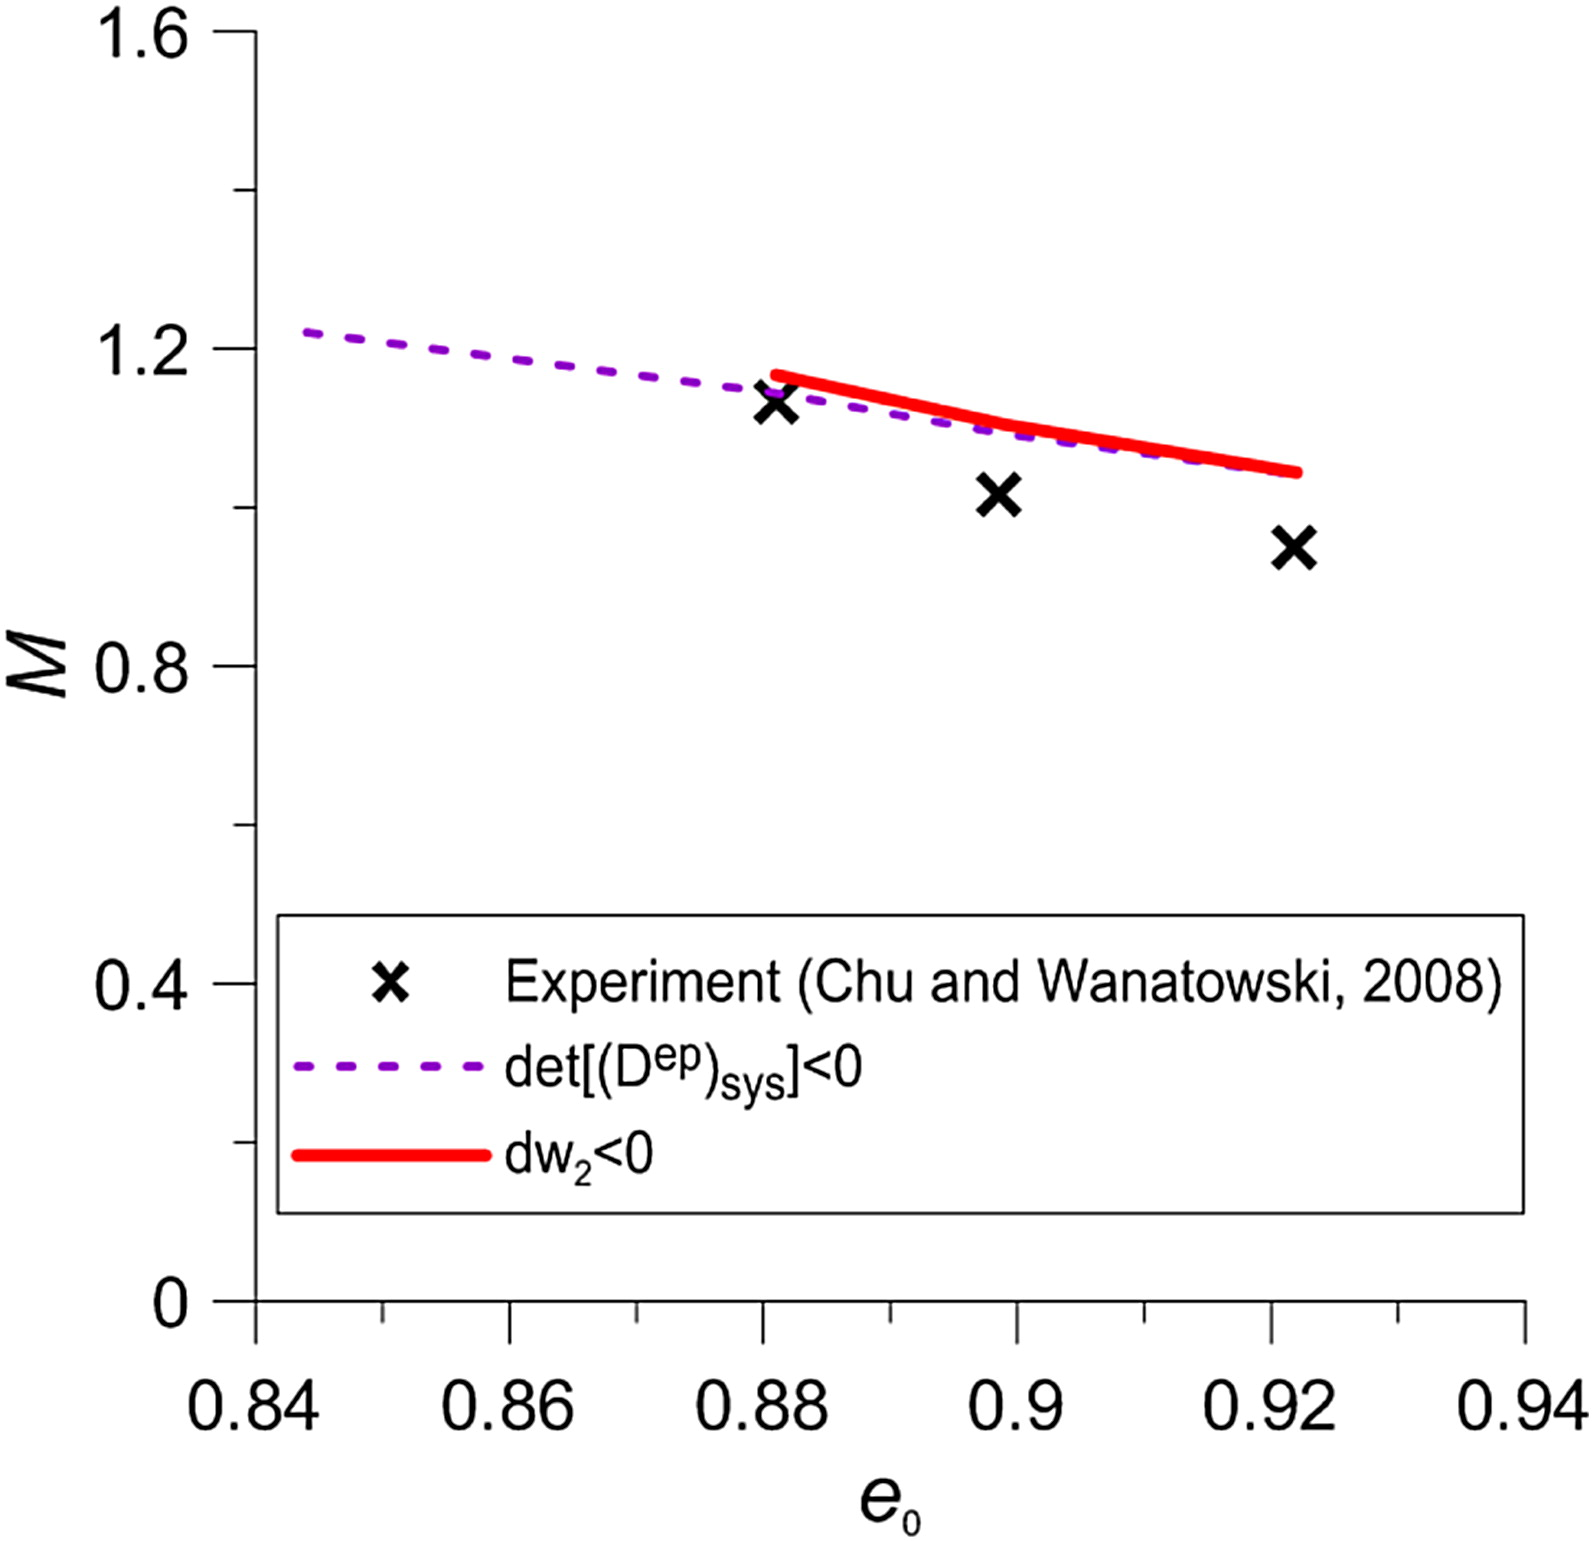
\includegraphics[width=\textwidth]{figures/figure13.jpg}
            \bicaption{Influence of the initial void ratio on the stress ratio at the onset of static liquefaction}{初始液化比对静态液化开始时应力比的影响}
            \label{figure:13}
        \end{figure}
    \end{minipage}
\end{figure}
    }

\end{ParaColumn}